\section{Remediation Strategies and October Validation}
\label{sec:remediation}

The practical choice is between changing a physical input to avoid a defective
pathway and correcting the rate assigned to surface-return water. The completed
experiments support the targeted correction as the more appropriate strategy,
but not an unconditional release claim. The candidate's routed hydrograph has
an unresolved volume inconsistency despite nearly unchanged water-yield ledgers.

\begin{table}[H]
\centering\small
\caption{Remediation options and current evidence boundary.}
\begin{tabular}{p{.20\textwidth}p{.34\textwidth}p{.35\textwidth}}
\toprule
Option & Mechanism & Disposition \\
\midrule
Raise initial roughness & Change depression storage and rainfall-excess timing;
some events leave the compressed-return path & Diagnostic workaround only;
changes runoff and resistance, with no universal safe threshold \\
Return-peak estimator & Use hourly return ledger, or daily return divided by
86,400 s; retain existing water-transfer path & Implemented, no new flags;
mutation improvement, unresolved watershed hydrograph closure \\
Fully coupled routing & Route combined rainfall excess and timed return with
consistent storage and recession bookkeeping & Earlier feasibility attempt
stopped at solver-contract failures; not the implemented candidate \\
\bottomrule
\end{tabular}
\end{table}

\subsection{What initial random roughness changes}

\texttt{rrinit} initialises random surface roughness, in metres. It is not
itself a reservoir depth or a return-flow duration. Current roughness
\texttt{rrc} contributes to depression storage in \texttt{IRS} and to surface
friction in \texttt{FRCFAC}; roughness and erosion feedback remain active.
The implemented depression-depth relation is
\begin{equation}
d_{\rm dep}=\max\{0,\;0.112r+3.1r^2-1.20rS\},
\end{equation}
where $r$ is current random roughness in metres and $S$ is slope as a fraction.
For a uniform 30\% slope, evaluating the formula at the initial roughness gives:

\begin{table}[H]
\centering
\caption{Illustrative depression depth at 30\% slope, before equivalent-plane
averaging or subsequent roughness evolution.}
\begin{tabular}{rrr}
\toprule
Initial roughness & Depression depth & Increase over 10 cm \\
\midrule
10 cm & 6.20 mm & --- \\
17 cm & 47.43 mm & 41.23 mm \\
60 cm & 967.20 mm & 961.00 mm \\
\bottomrule
\end{tabular}
\end{table}

These depths are not storage through which all watershed streamflow must pass.
\texttt{GRNA} applies depression storage to rainfall excess; sufficiently large
storage can remove that excess event. The subsequent soil-water balance can
still return water from a full profile through \surdra{}, without applying the
same depression-storage subtraction again. Lateral flow and groundwater
baseflow are also not routed through this rainfall-excess storage calculation.
Consequently, a very large nominal storage increase need not remove a
comparable depth of total streamflow.

In the original return branch, positive rainfall-excess duration makes the
imposed return rate equal to daily return divided by that duration. Eliminating
positive excess can move the calculation to a different return-duration path:
storm duration, upslope duration, or ultimately 24 hours. This can prevent an
anomalous peak without eliminating surface return or repairing its timing.
It can also change the selected peak solver. Raising roughness does not
guarantee a monotonic reduction of peaks.

Anurag's email identifies 17 cm as a threshold in his undisturbed-forest
comparison, after initially testing 60 cm against a 6 cm baseline. That is a
case-specific transition, not a WEPP constant or a physical discontinuity at
17 cm. Its exact event mechanism requires tracing the operands. His
burned--unburned comparison also changes other scenario properties; it is not
the matched roughness-only Cedar Creek experiment below. The embedded screenshot
was not available in the retained text attachment, so no quantitative claim
about its axes, aggregation, or executable identity is made here.

The disturbed templates examined during this investigation are not described
by a single universal 6 cm default. OldForest is 10 cm unburned, 4 cm at low
severity, and 6 cm at moderate and high severity; shrub is 6 cm throughout,
and tall grass is 2 cm throughout. The unburned
\texttt{hand-to-mouth-drought} landscape is predominantly shrub (92.67\%),
explaining its 6 cm value. The 10 cm records in
\texttt{warming-championship} are consistent with the existing forest template;
they are not evidence that Marta changed the default.

\paragraph{External consequences of roughness inflation.}
Changing roughness changes rainfall-excess onset, duration and volume,
hydraulic resistance, and potentially erosion and downstream synchronisation.
It therefore changes the scientific scenario in addition to changing exposure
to the defect. Burned--unburned peak ordering is not sufficient justification
for selecting a roughness value, and numerical stabilisation is not evidence
that a larger roughness is physically appropriate. Fire-related loss of litter
or microtopographic storage must be evaluated as a separate parameterisation
question; no universal roughness response by burn severity is inferred here.
The 17 and 60 cm values are diagnostic interventions, not recommended defaults.

\subsection{The implemented parameter-free return-peak correction}

The candidate adds \texttt{SURPEAK} and its integration in \texttt{IRS}. It
changes peak assignment, not the existing daily surface-return transfer or the
depression-storage parameterisation. It introduces no user parameter or flag.
For non-hourly water balance, the estimator is
\begin{equation}
q_{\rm candidate}=q_{\rm rain}+R/86{,}400,
\end{equation}
where $R$ is daily returned depth and rates use compatible depth/time units.
Spreading return over 24 hours is a simple explicit assumption when subdaily
timing is unavailable. It can understate a brief return pulse; it is not a
validated physical return duration or a claim of instantaneous peak accuracy.

With hourly water balance, the estimator uses the existing hourly return
ledger and a volume-closing hourly rainfall-excess distribution. It adds the
increase in maximum hourly forcing caused by return to the rain-only routed
peak, bounded below by the maximum hourly return rate. Its result lies between
$\max(q_{\rm rain},q_{\rm return,max})$ and
$q_{\rm rain}+q_{\rm return,max}$. Return is not separately attenuated through a
fully coupled kinematic-wave calculation. This bounded estimator is deliberately
less ambitious than the abandoned direct-coupling patch described above.

The existing OFE water-transfer and contour paths remain in place. Altered
peaks may still change erosion, rill-width feedback, and channel routing;
unchanged intended water accounting does not imply byte-identical output.
The release-source audit found 485 source/include/build files matching the
retained unpatched tree after normalising the build system's capacity-include
swap. Candidate differences are confined to \texttt{irs.for},
\texttt{surpeak.for}, and \texttt{makefile}. Complete executable hashes and
the compiler-provenance limitation remain in the evidence packages
\cite{mutationredo,rrlegacy}.

\subsection{Repeated Topanga mutation study}

The \texttt{hand-to-mouth-drought} repeat completed all 280 baselines and
1,088 eligible mutations over 45 years, with the candidate on both sides of
each pair. It retained the original $\pm1\%$ \Ksat{} and $\pm0.01$ paired-cover
probes and did not change roughness or depression storage. Shared inputs match
the original census byte-for-byte. The historical comparison is nevertheless
descriptive, not a same-lineage patch-only causal estimate: source lineage and
observation grain differ \cite{mutationredo}.

\begin{table}[H]
\centering\small
\caption{Candidate-build mutation response. Denominators apply to each
response's eligible positive pairs, not independent storms or hillslopes.}
\begin{tabular}{lrrr}
\toprule
Response & Positive pairs & Outside 0.5--2 & Outside 0.2--5 \\
\midrule
Runoff depth & 218,974 & 453 (0.207\%) & 34 (0.016\%) \\
Sediment delivery & 128,469 & 372 (0.290\%) & 90 (0.070\%) \\
Peak rate & 200,932 & 1,021 (0.508\%) & 218 (0.108\%) \\
\bottomrule
\end{tabular}
\end{table}

The fivefold peak-departure rate falls from 604/199,086 (0.303\%) in August
to 218/200,932 (0.108\%). The high-rate scatter is visibly tighter, and the
remaining fivefold tail reaches only 17.39 mm/h on the baseline side and
21.29 mm/h on the mutant side. In the central 0.5--2 band at baseline peaks
of 30--100 mm/h, \Ksat{} incongruence falls from 24.1\% to 4.68\% unburned
and from 26.0\% to 2.24\% burned, using the original convention including ties.
These findings support the observed reduction and downward shift of the most
conspicuous departures.

They do not support saying that all sensitivity decreased. Twofold peak
departures remain at 0.508\%, versus 0.497\% originally; 594 of the 1,021
current twofold departures retain runoff within 5\% of baseline. Sediment's
twofold-tail rate rises from 0.195\% to 0.290\%. Of the 218 remaining fivefold
peak departures, 184 have no return in either run, the same no-return count
reported originally. Residual rows are screening candidates, not individually
adjudicated defects.

\begin{figure}[p]
\centering
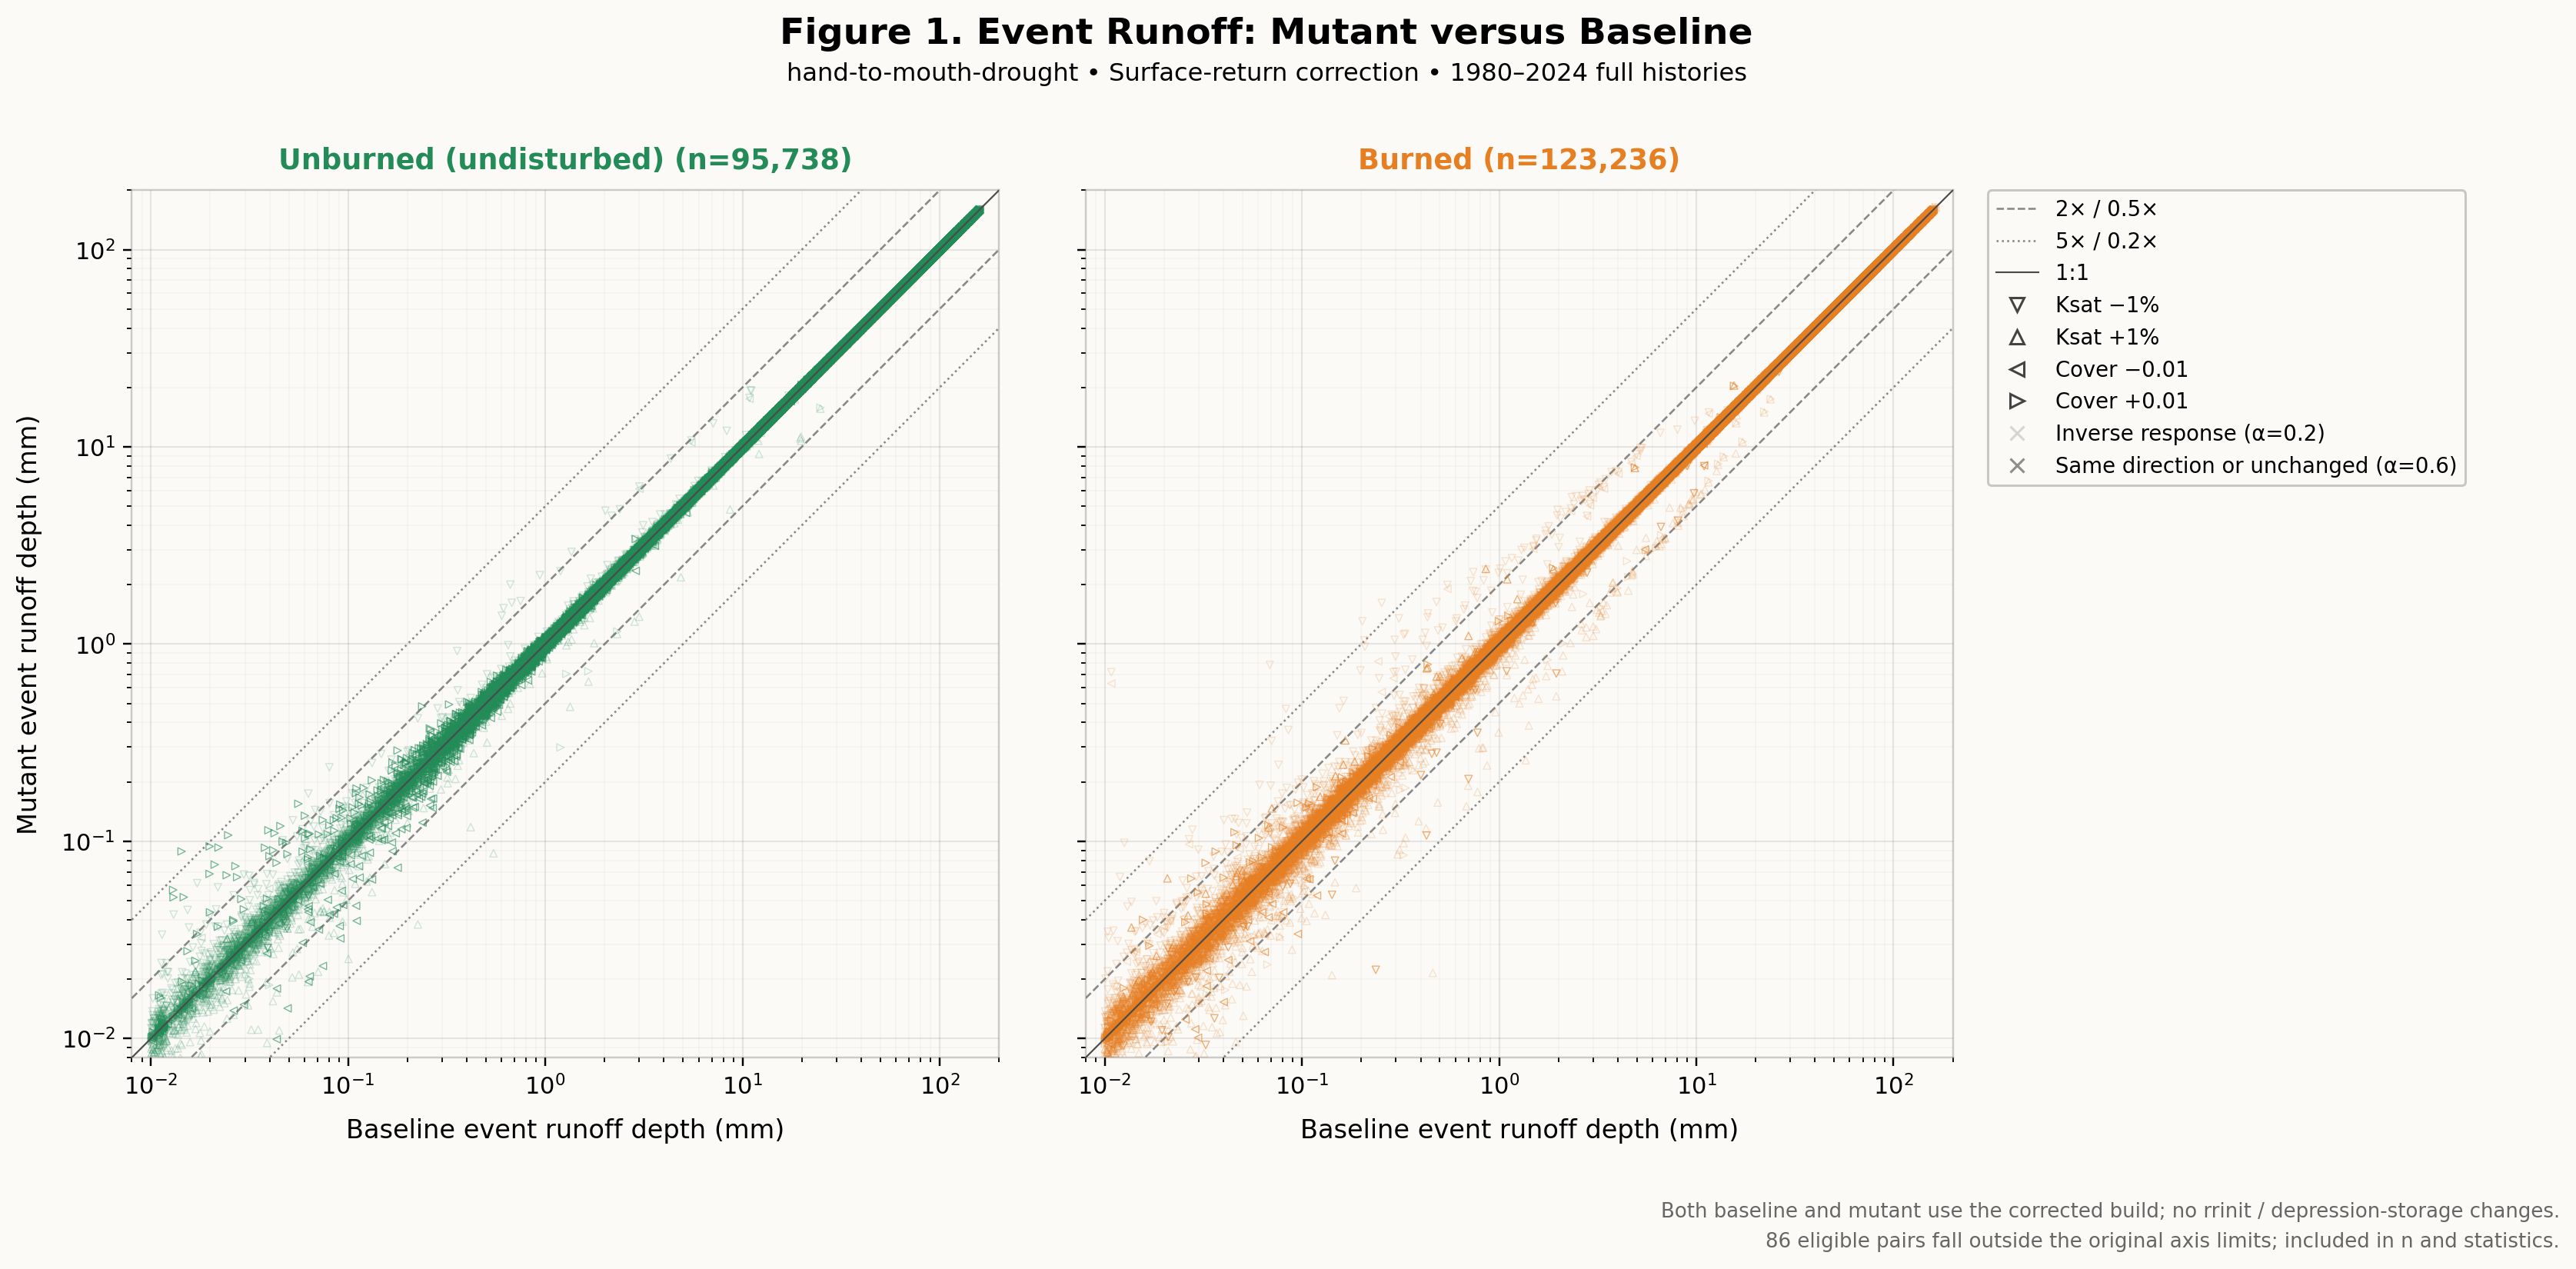
\includegraphics[width=\textwidth,height=.78\textheight,keepaspectratio]{../../work-packages/20261006_surface_return_mutation/artifacts/figure-1.png}
\caption{Candidate-build runoff response to the original
small mutations. Original floors, markers and ratio guides are retained.
Statistics include 86 eligible pairs outside the displayed axis bounds.}
\label{fig:redo-runoff}
\end{figure}
\begin{figure}[p]
\centering
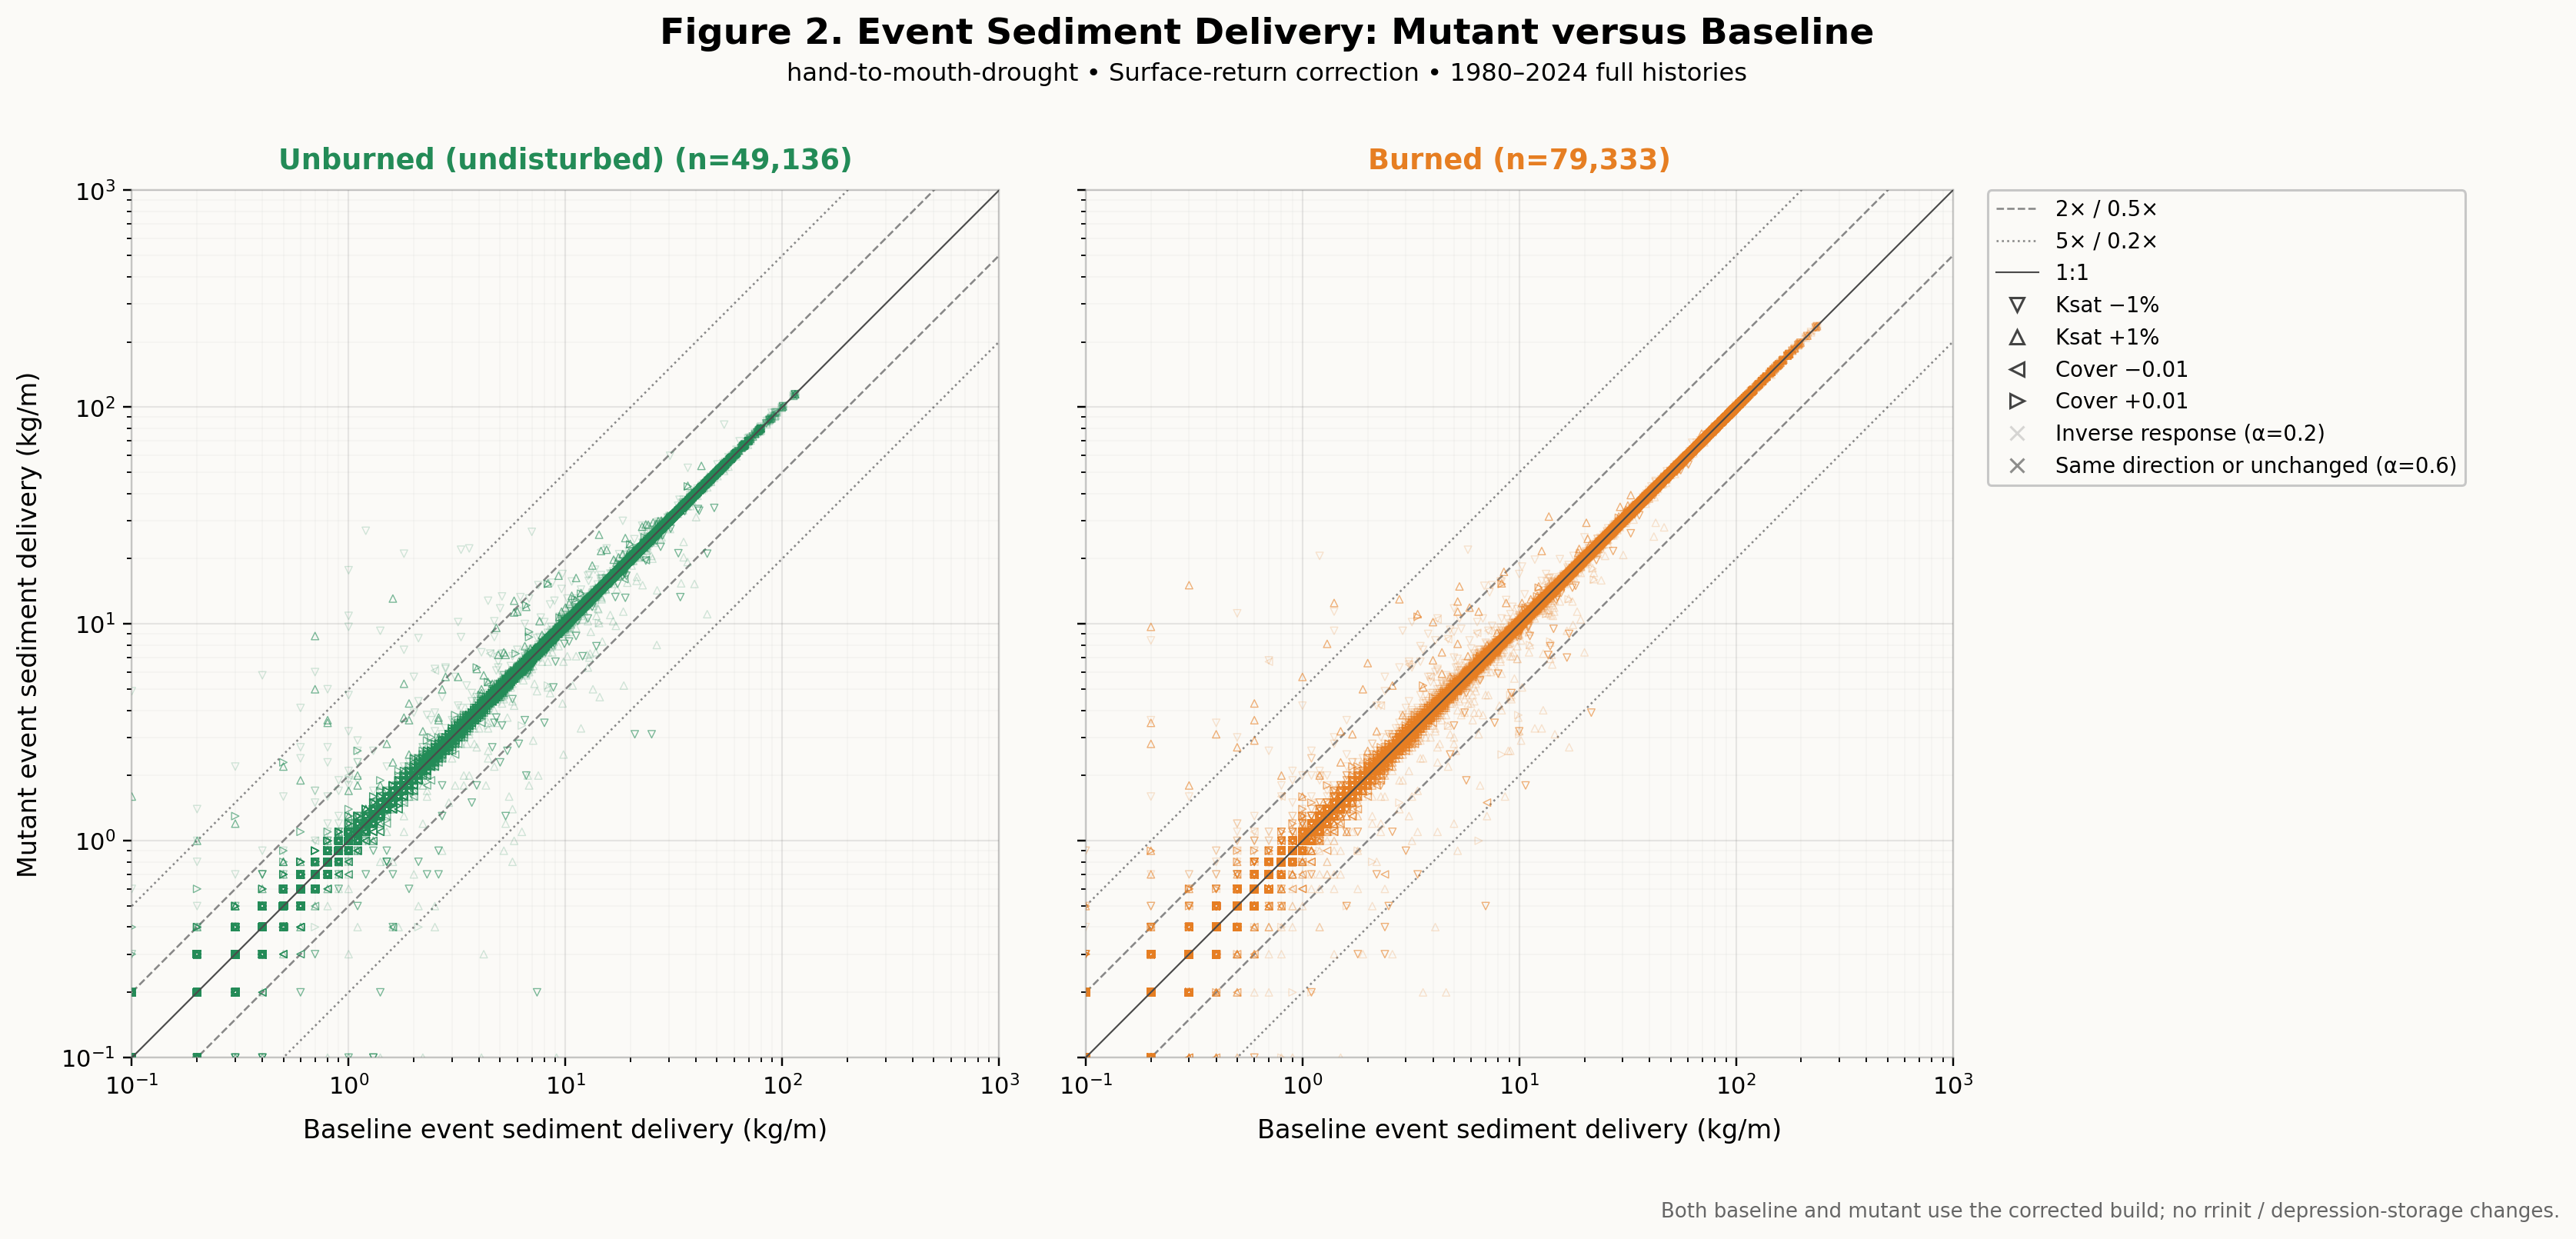
\includegraphics[width=\textwidth,height=.78\textheight,keepaspectratio]{../../work-packages/20261006_surface_return_mutation/artifacts/figure-2.png}
\caption{Candidate-build event sediment delivery.
Printed sediment is quantised to 0.1 kg/m; 70,424 plotted pairs are exact
ties. The ledger separately retains 549 baseline-positive-only and 619
mutant-positive-only sediment rows rather than hiding event changes.}
\label{fig:redo-sediment}
\end{figure}
\begin{figure}[p]
\centering
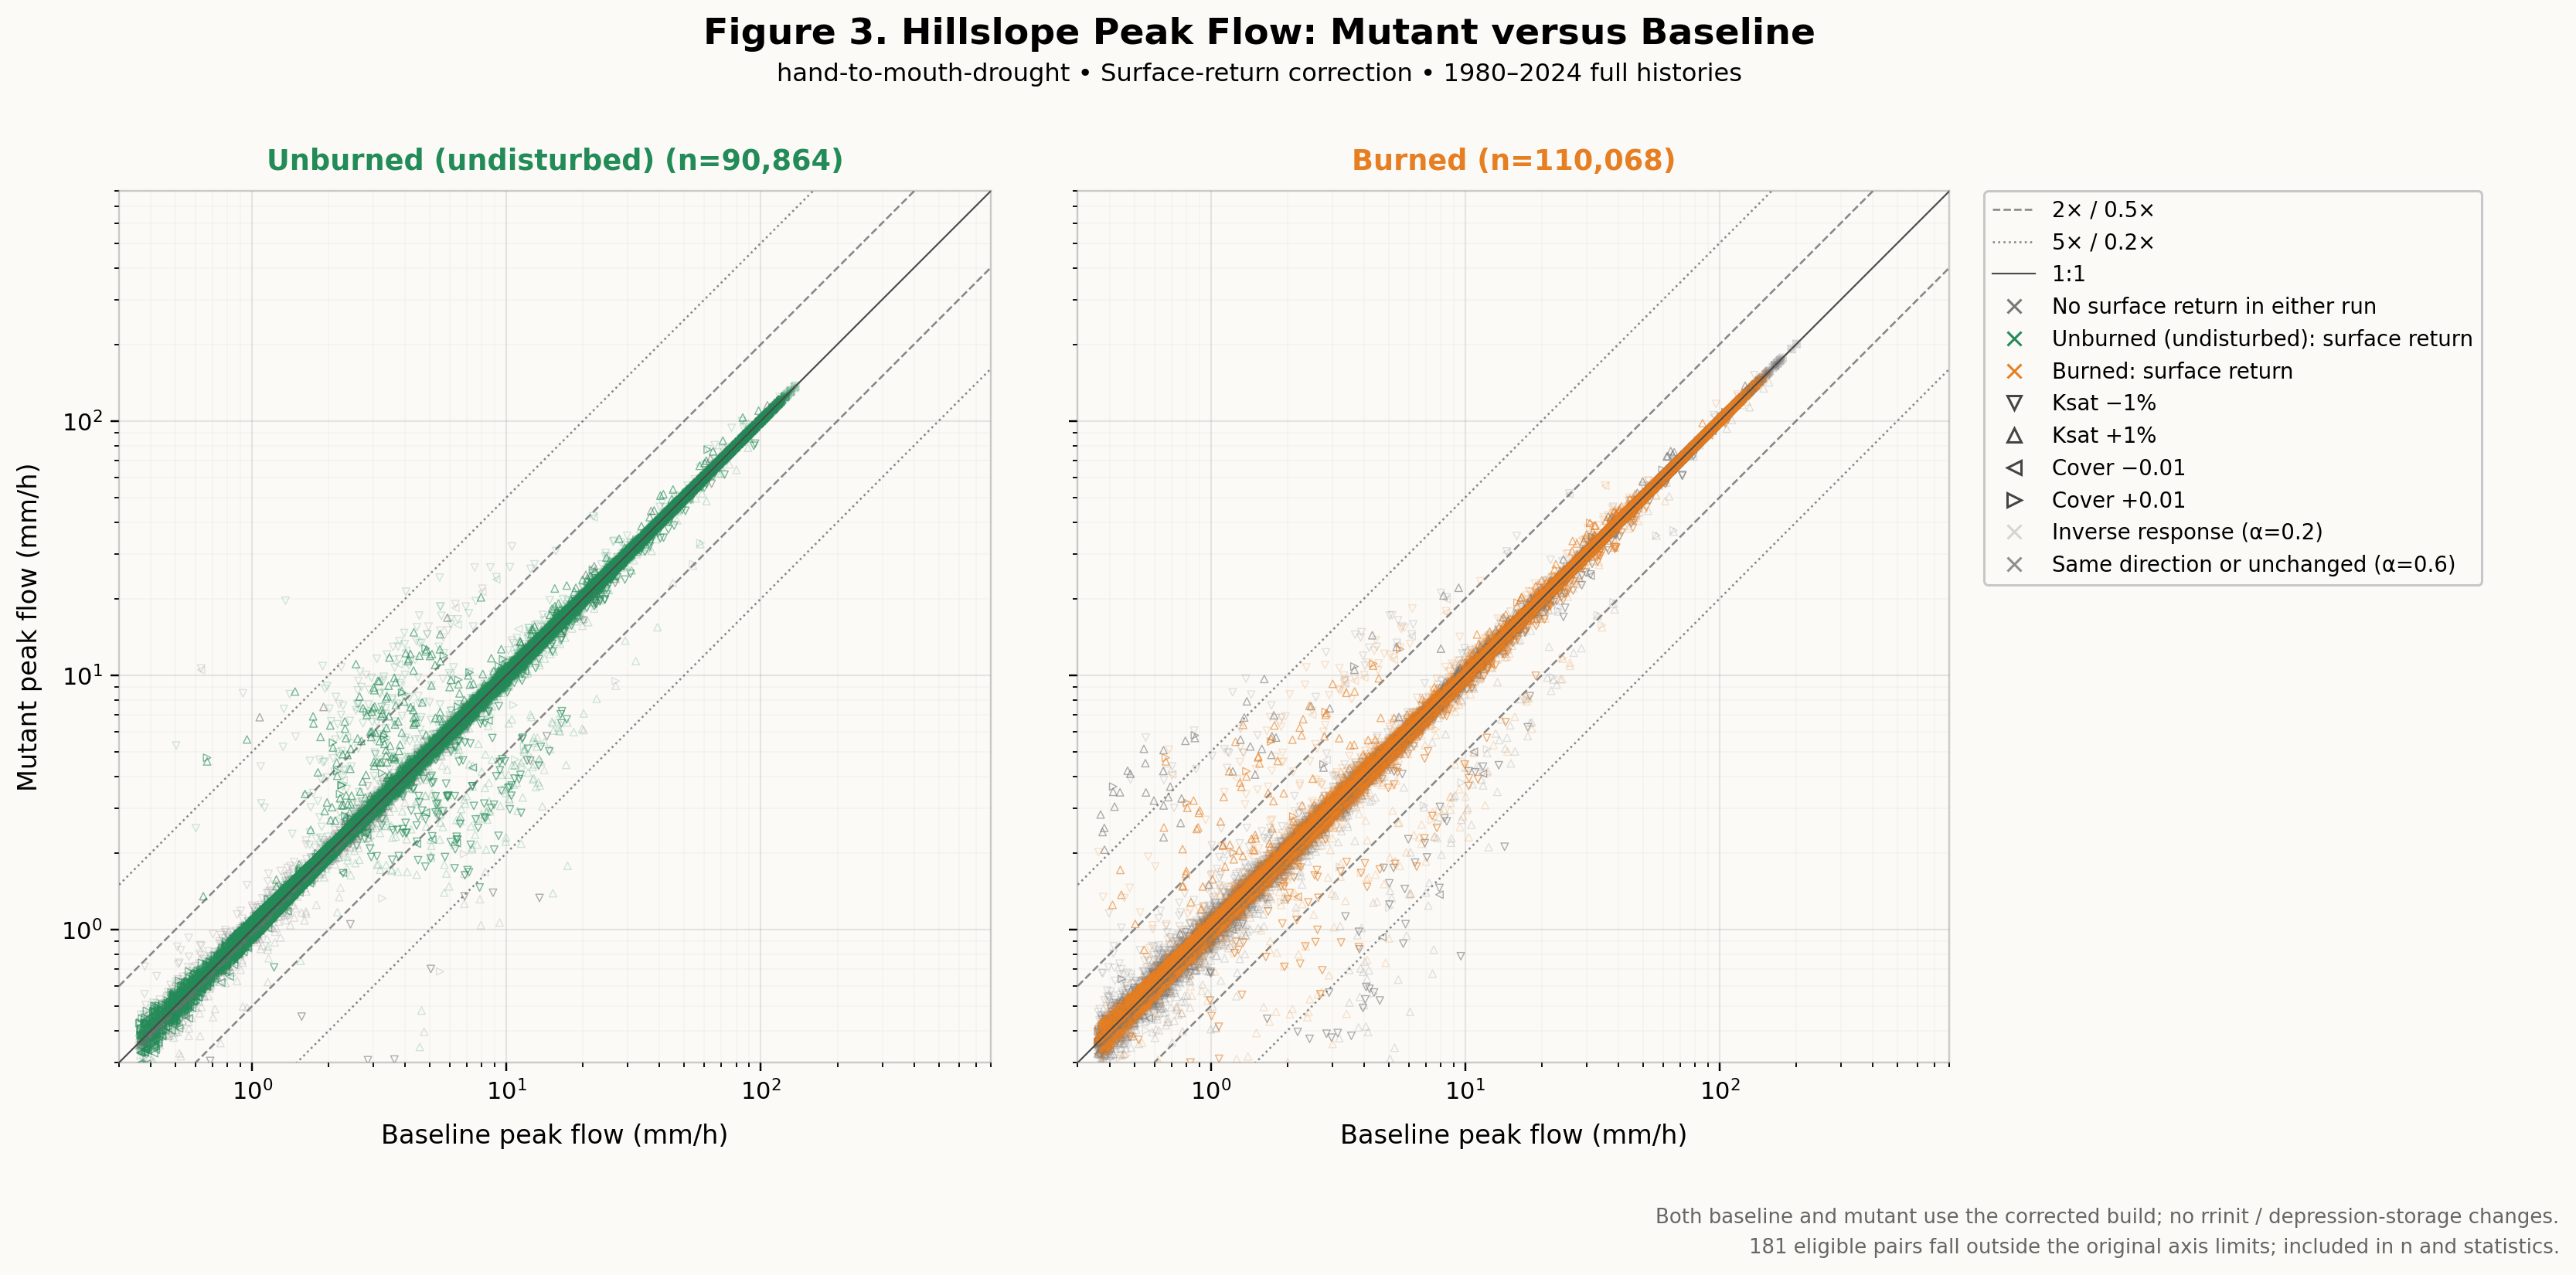
\includegraphics[width=\textwidth,height=.78\textheight,keepaspectratio]{../../work-packages/20261006_surface_return_mutation/artifacts/figure-3.png}
\caption{Candidate-build hillslope peak response.
The severe high-rate tail is reduced, not eliminated. Statistics include 181
eligible pairs outside the original axis bounds. Both members of every pair
use the candidate; this is not a direct original-versus-candidate scatter.}
\label{fig:redo-peak}
\end{figure}
\clearpage

\subsection{Cedar Creek watershed and roughness experiment}

The \texttt{warming-championship} run on forest is titled Cedar Creek and
contains 864 hillslopes, 1,904 OFEs, 371 channels and outlet element 1235.
All 24 years, 1980--2003, including initialisation, were rerun. Only the
1,885 initial-condition roughness records originally at 10 cm were changed
to 17 or 60 cm. Two 6 cm and seventeen 0.8 cm records were preserved. Soil,
climate, cover, hourly water balance and channel parameters were held fixed.
This is a roughness intervention, not a burned--unburned comparison.

Each build comparison comprises 2,592 hillslope executions, three watershed
executions and one channel-output-mode control, all successful. The observer
requests full 600-second discharge without changing the routing timestep;
seven canonical watershed outputs are byte-identical between observer and
original output mode. All 14 untouched hillslope controls pass. Each main
lane contains 8,766 days and 1,262,304 discharge samples. Original project
inputs remain unchanged. The legacy experiment uses verified
\texttt{wepp\_260803} and \texttt{wepp\_260803\_hill} binaries with inputs
matching each candidate lane exactly \cite{rrfixed,rrlegacy}.

\begin{table}[H]
\centering\small
\caption{Daily outlet-peak departures from each build's own 10 cm case.
These ranges are not changes in the single largest simulation peak.}
\begin{tabular}{llrrr}
\toprule
Build & Roughness & Minimum & Maximum & Days with $|\Delta|>1\%$ \\
\midrule
Original & 17 cm & $-18.2345\%$ & $+4.8352\%$ & 26 \\
Candidate & 17 cm & $-1.5996\%$ & $+0.4515\%$ & 2 \\
Original & 60 cm & $-18.2345\%$ & $+4.7757\%$ & 61 \\
Candidate & 60 cm & $-2.5049\%$ & $+0.5672\%$ & 3 \\
\bottomrule
\end{tabular}
\end{table}

The original build is sensitive to roughness: on November 6, 1983 its daily
peak falls from 1.36176 to 1.11345 m$^3$/s at both 17 and 60 cm. That shared
response is consistent with crossing a threshold, but is not an event-level
trace of its cause. Some physical roughness sensitivity should remain after
repair. The candidate reduces the extreme outlet sensitivity here, not all
hillslope relative sensitivities or their frequency. Small denominators and
different screened populations matter at hillslope scale.

Whole-record outlet-volume reductions are almost identical across builds:
approximately 0.01098\% at 17 cm and 0.02106\% at 60 cm. Candidate maximum
daily peaks are 43.06409, 42.77490 and 42.67082 m$^3$/s for 10/17/60 cm,
all on April 27, 1990. Original maxima are 50.50288, 50.47683 and
50.53258 m$^3$/s: increasing roughness does not uniformly lower the maximum.

\begin{figure}[p]
\centering
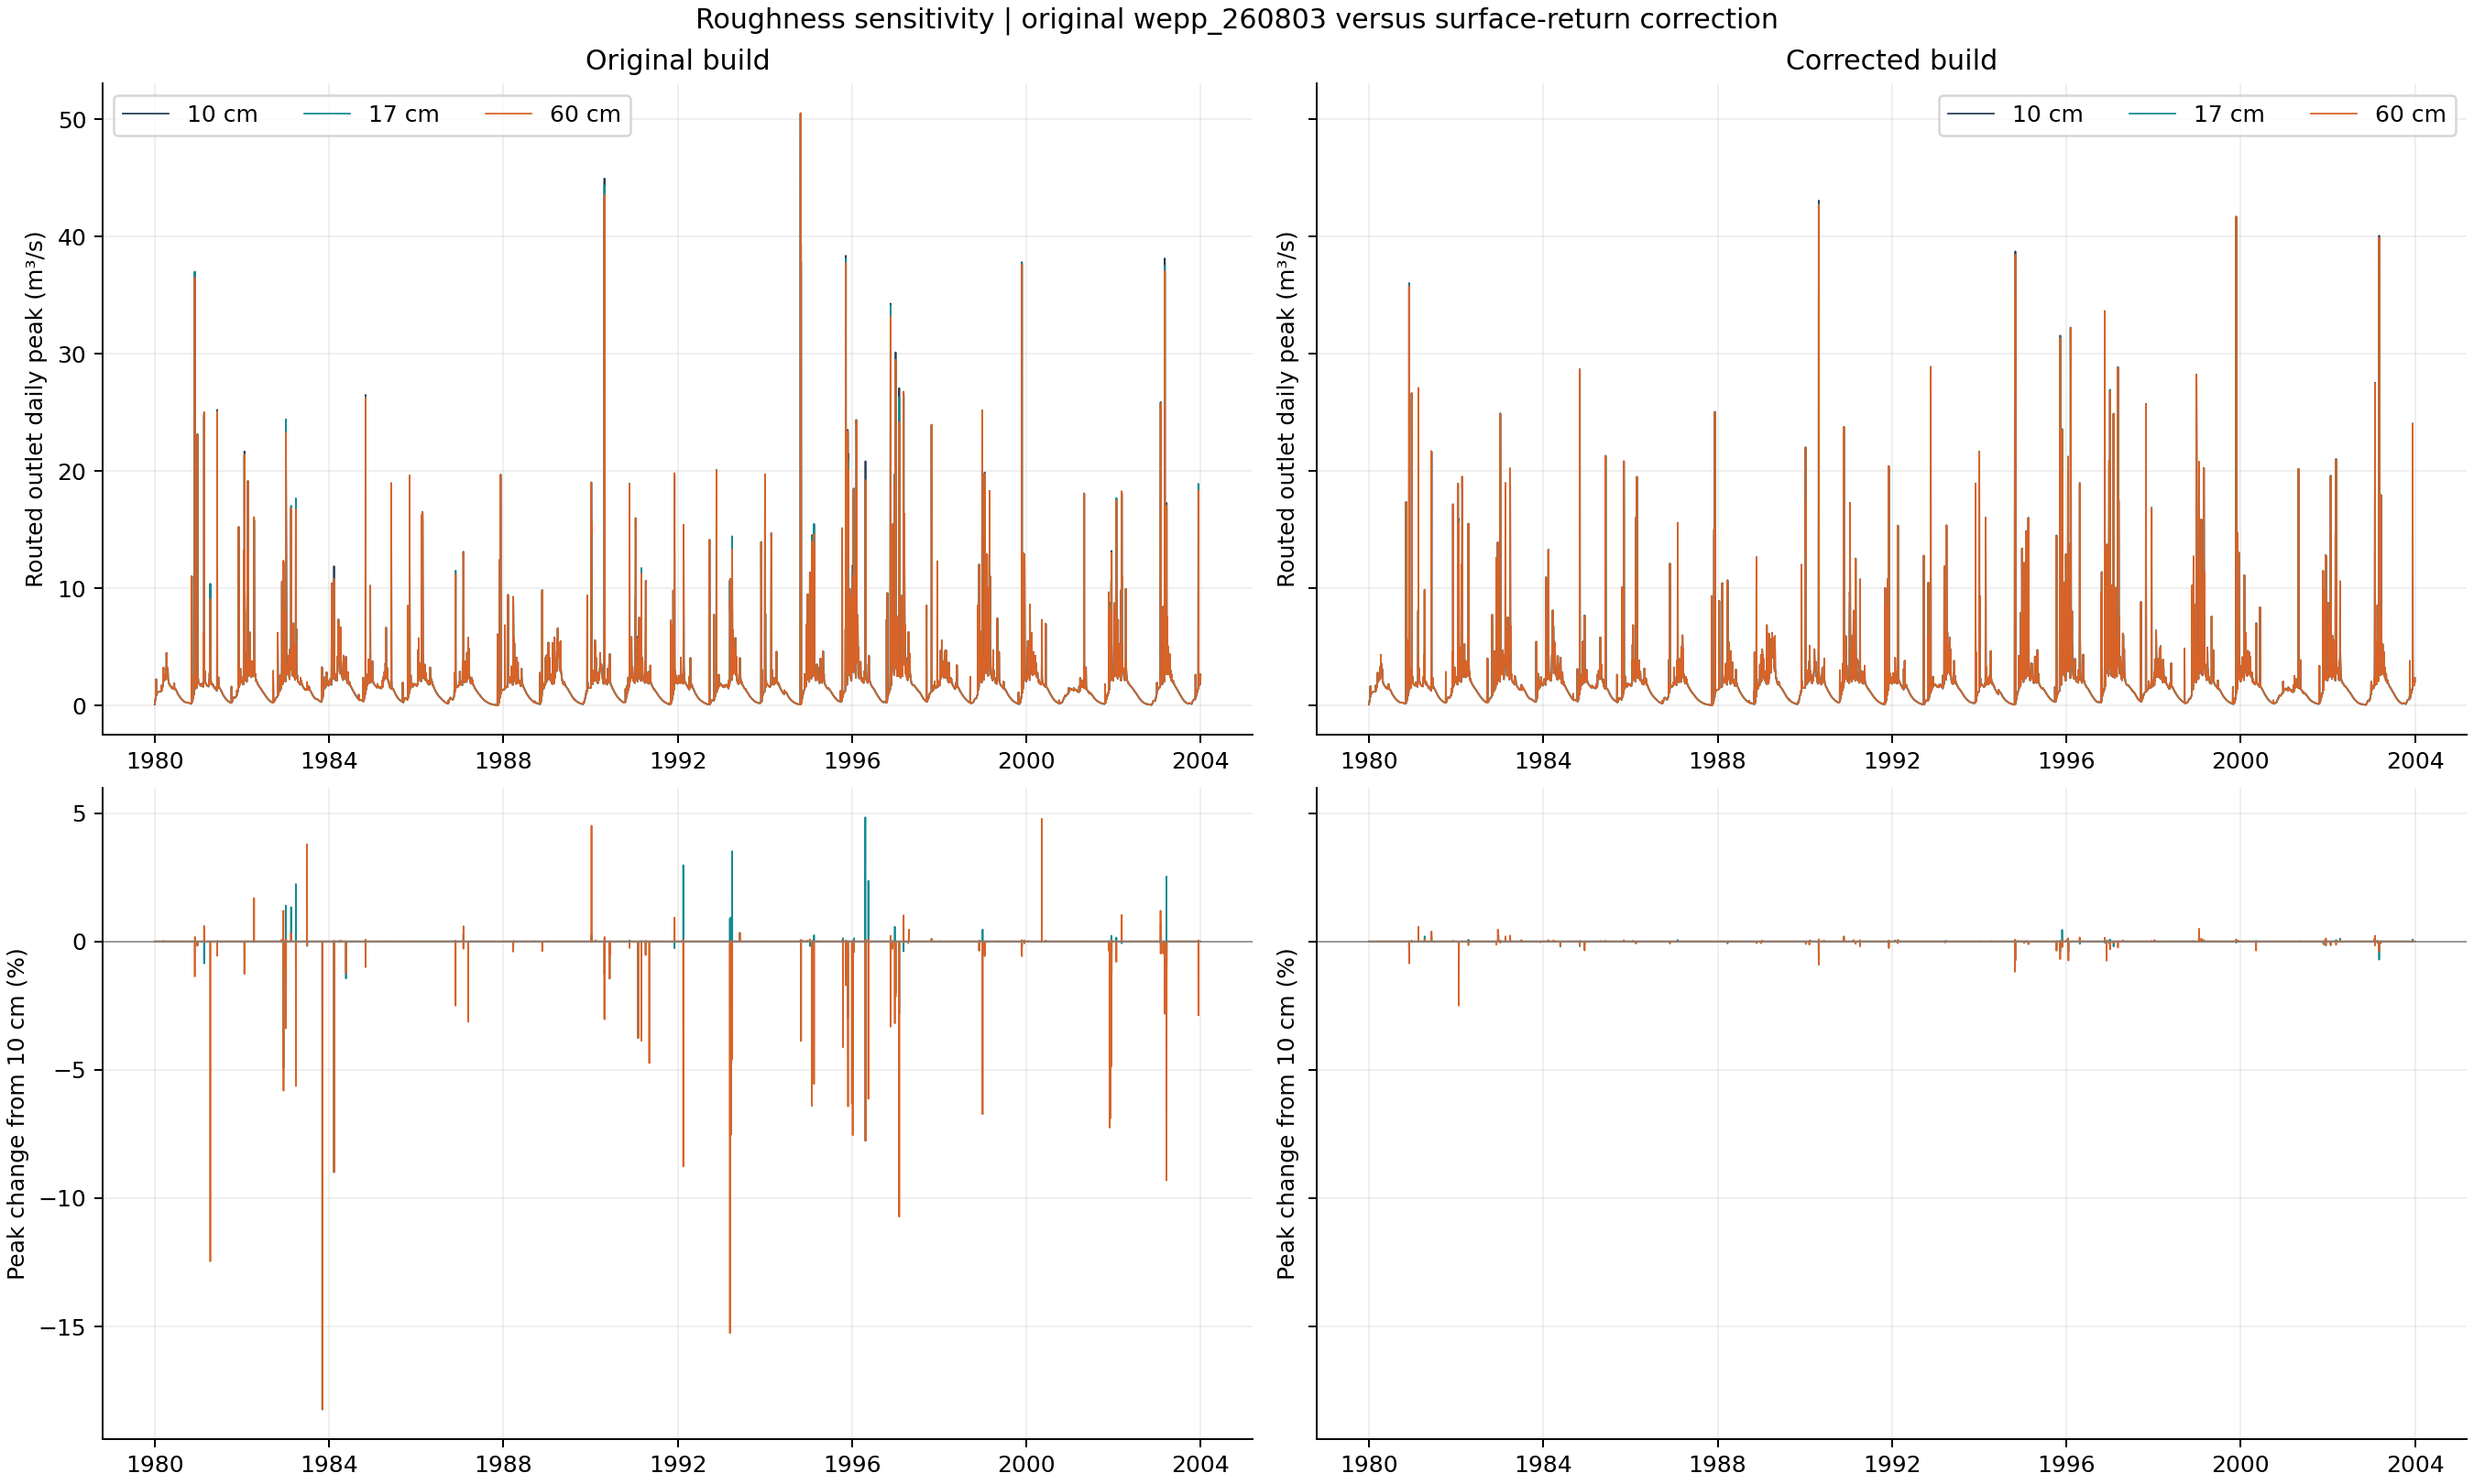
\includegraphics[width=\textwidth,height=.78\textheight,keepaspectratio]{../../work-packages/20261006_warming_rrinit_legacy/artifacts/comparison/figure-1-build-roughness.png}
\caption{Within-build roughness sensitivity at Cedar Creek. Shared vertical
scales distinguish the original and candidate responses without changing
the reference case between roughness lanes.}
\label{fig:roughness-builds}
\end{figure}

\subsection{Totalwatsed yield is not the routed outlet hydrograph}

Freshly rebuilt \texttt{totalwatsed} streamflow is PASS surface runoff plus
bottom-OFE lateral flow plus postprocessed groundwater baseflow. It is a daily,
pre-channel yield measure, not an instantaneous routed outlet discharge.
The retained groundwater settings use zero initial storage, a 0.04/day
baseflow coefficient, and zero deep seepage. The watershed area is
19,258,143.09 m$^2$.

\begin{table}[H]
\centering\small
\caption{Candidate-build totalwatsed streamflow. Daily mean rates cannot
resolve within-day peak or travel-time changes.}
\begin{tabular}{rrrr}
\toprule
Roughness & Total volume (million m$^3$) & Mean annual depth (mm) & Max daily mean (m$^3$/s) \\
\midrule
10 cm & 1267.7357 & 2742.8563 & 28.7701 \\
17 cm & 1267.5960 & 2742.5542 & 28.5946 \\
60 cm & 1267.4677 & 2742.2766 & 28.1919 \\
\bottomrule
\end{tabular}
\end{table}

At 10 cm, annual component depths are approximately 416.36 mm surface runoff,
874.85 mm lateral flow and 1451.65 mm baseflow. About 85\% of this streamflow
therefore comes from the latter two components. Combined with the separation
between depression storage and soil-water return, this helps explain why
967 mm of nominal depression depth does not remove a comparable depth of
streamflow. It does not demonstrate negligible roughness effects in every
hillslope or watershed.

The three candidate daily-yield series almost overlap. Total yields change
by $-0.01102\%$ and $-0.02113\%$ at 17 and 60 cm. A sensitivity-focused
selection of smaller totalwatsed events (lower-half local peaks, separated
by at least seven days, prominence at least 0.1 m$^3$/s) found example
daily departures of roughly $-0.14\%$ to $-0.23\%$. This small
\emph{within-candidate roughness} response should not be confused with the
large \emph{between-build} smaller-event peak changes below.

\begin{figure}[p]
\centering
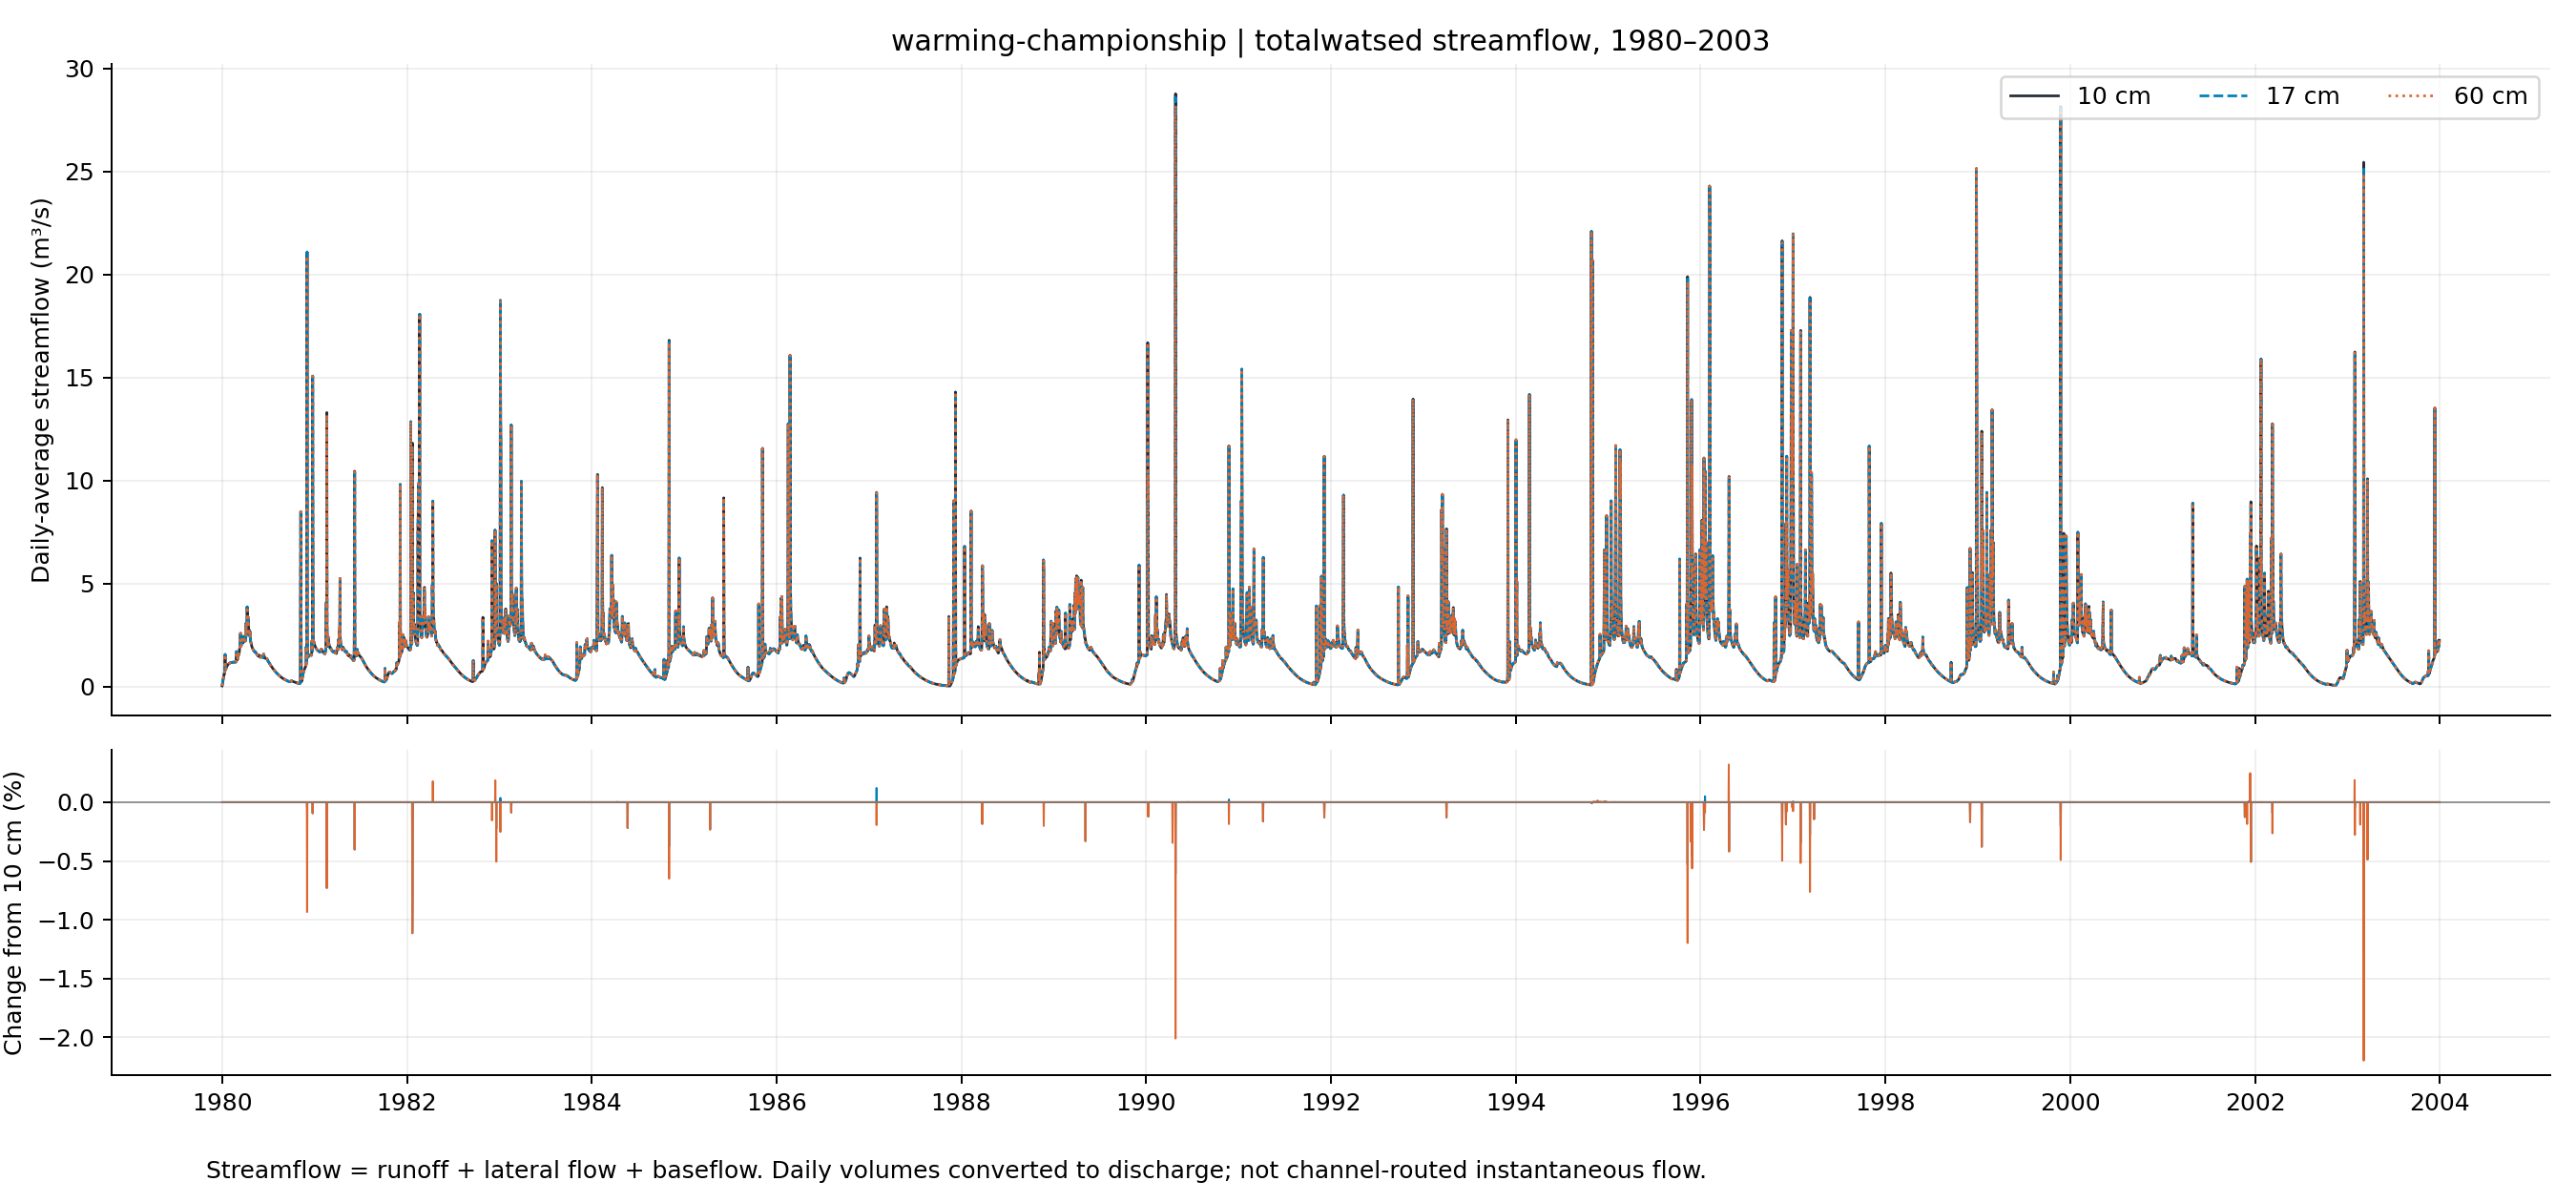
\includegraphics[width=\textwidth,height=.76\textheight,keepaspectratio]{artifacts/remediation-report/totalwatsed-hydrograph.png}
\caption{Candidate-build totalwatsed streamflow for all three roughness
values, expressed as daily mean flow. The lower panel exposes differences
hidden by near-overlapping series; these are not routed subdaily hydrographs.}
\label{fig:totalwatsed-full}
\end{figure}
\begin{figure}[p]
\centering
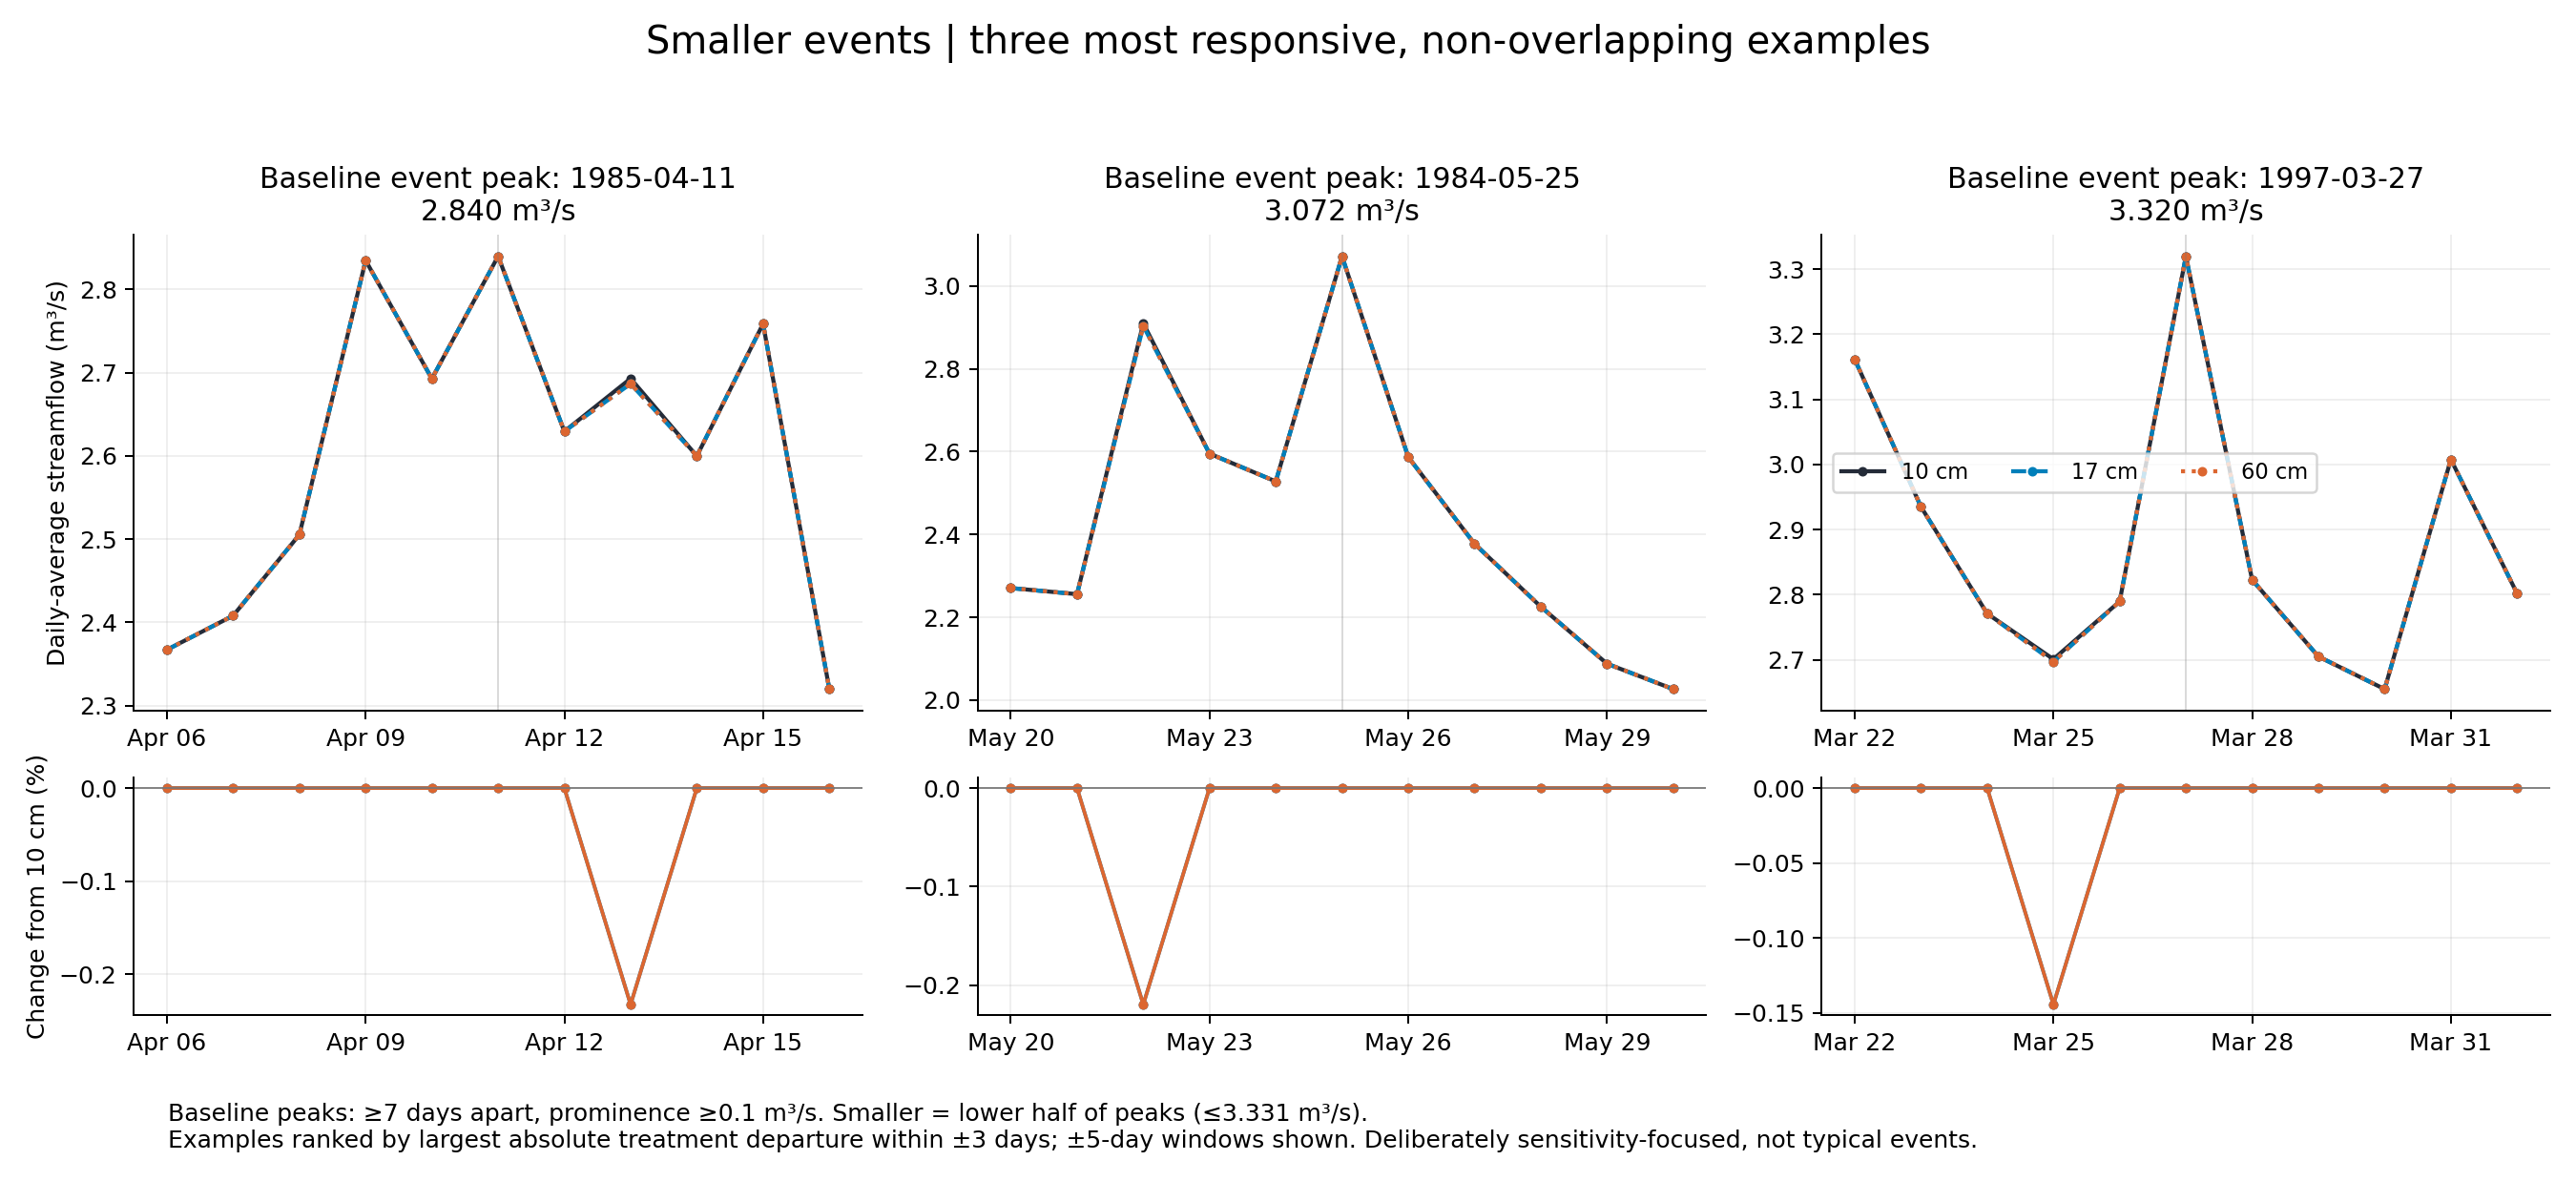
\includegraphics[width=\textwidth,height=.76\textheight,keepaspectratio]{artifacts/remediation-report/totalwatsed-smaller-events.png}
\caption{Sensitivity-focused smaller totalwatsed events under the candidate.
The daily-yield peak cutoff is 3.3311 m$^3$/s. Selection ranks departures
within three days of eligible peaks and displays five days on either side;
it differs from the outlet-peak selection used in Figure~\ref{fig:small-builds}.}
\label{fig:totalwatsed-small}
\end{figure}

\subsection{Matched 10 cm original versus candidate}

At unchanged 10 cm inputs, candidate totalwatsed yield differs by only
$+0.305$ m$^3$ out of 1.2677 billion m$^3$. Only 106 of 7,573,824 hillslope
daily runoff-volume records differ at printed precision, by at most 0.1 m$^3$;
392,667 hillslope peak records change. H352 on January 31, 1995 retains
4,077 m$^3$ while its peak changes from 4.0447 to 0.10625 m$^3$/s.
This confirms separation of volume from rate assignment, not physical accuracy
of either rate. Other peaks increase.

At the outlet, 2,356 daily peaks differ by more than 1\%, with departures
from $-46.97\%$ to $+156.00\%$. There are 1,930 lower, 2,417 higher and
4,419 unchanged daily peaks at printed precision. The original record maximum
is 50.50288 m$^3$/s on October 27, 1994; the candidate is 35.45196 m$^3$/s
that day. The candidate's own record maximum, 43.06409 m$^3$/s, occurs on a
different date. The outlet-volume ledger changes by just $-4.25$ m$^3$ over
24 years, but individual daily volumes are not invariant: 44 days change by
more than 1\%, spanning $-8.62\%$ to $+2.57\%$.

\begin{figure}[p]
\centering
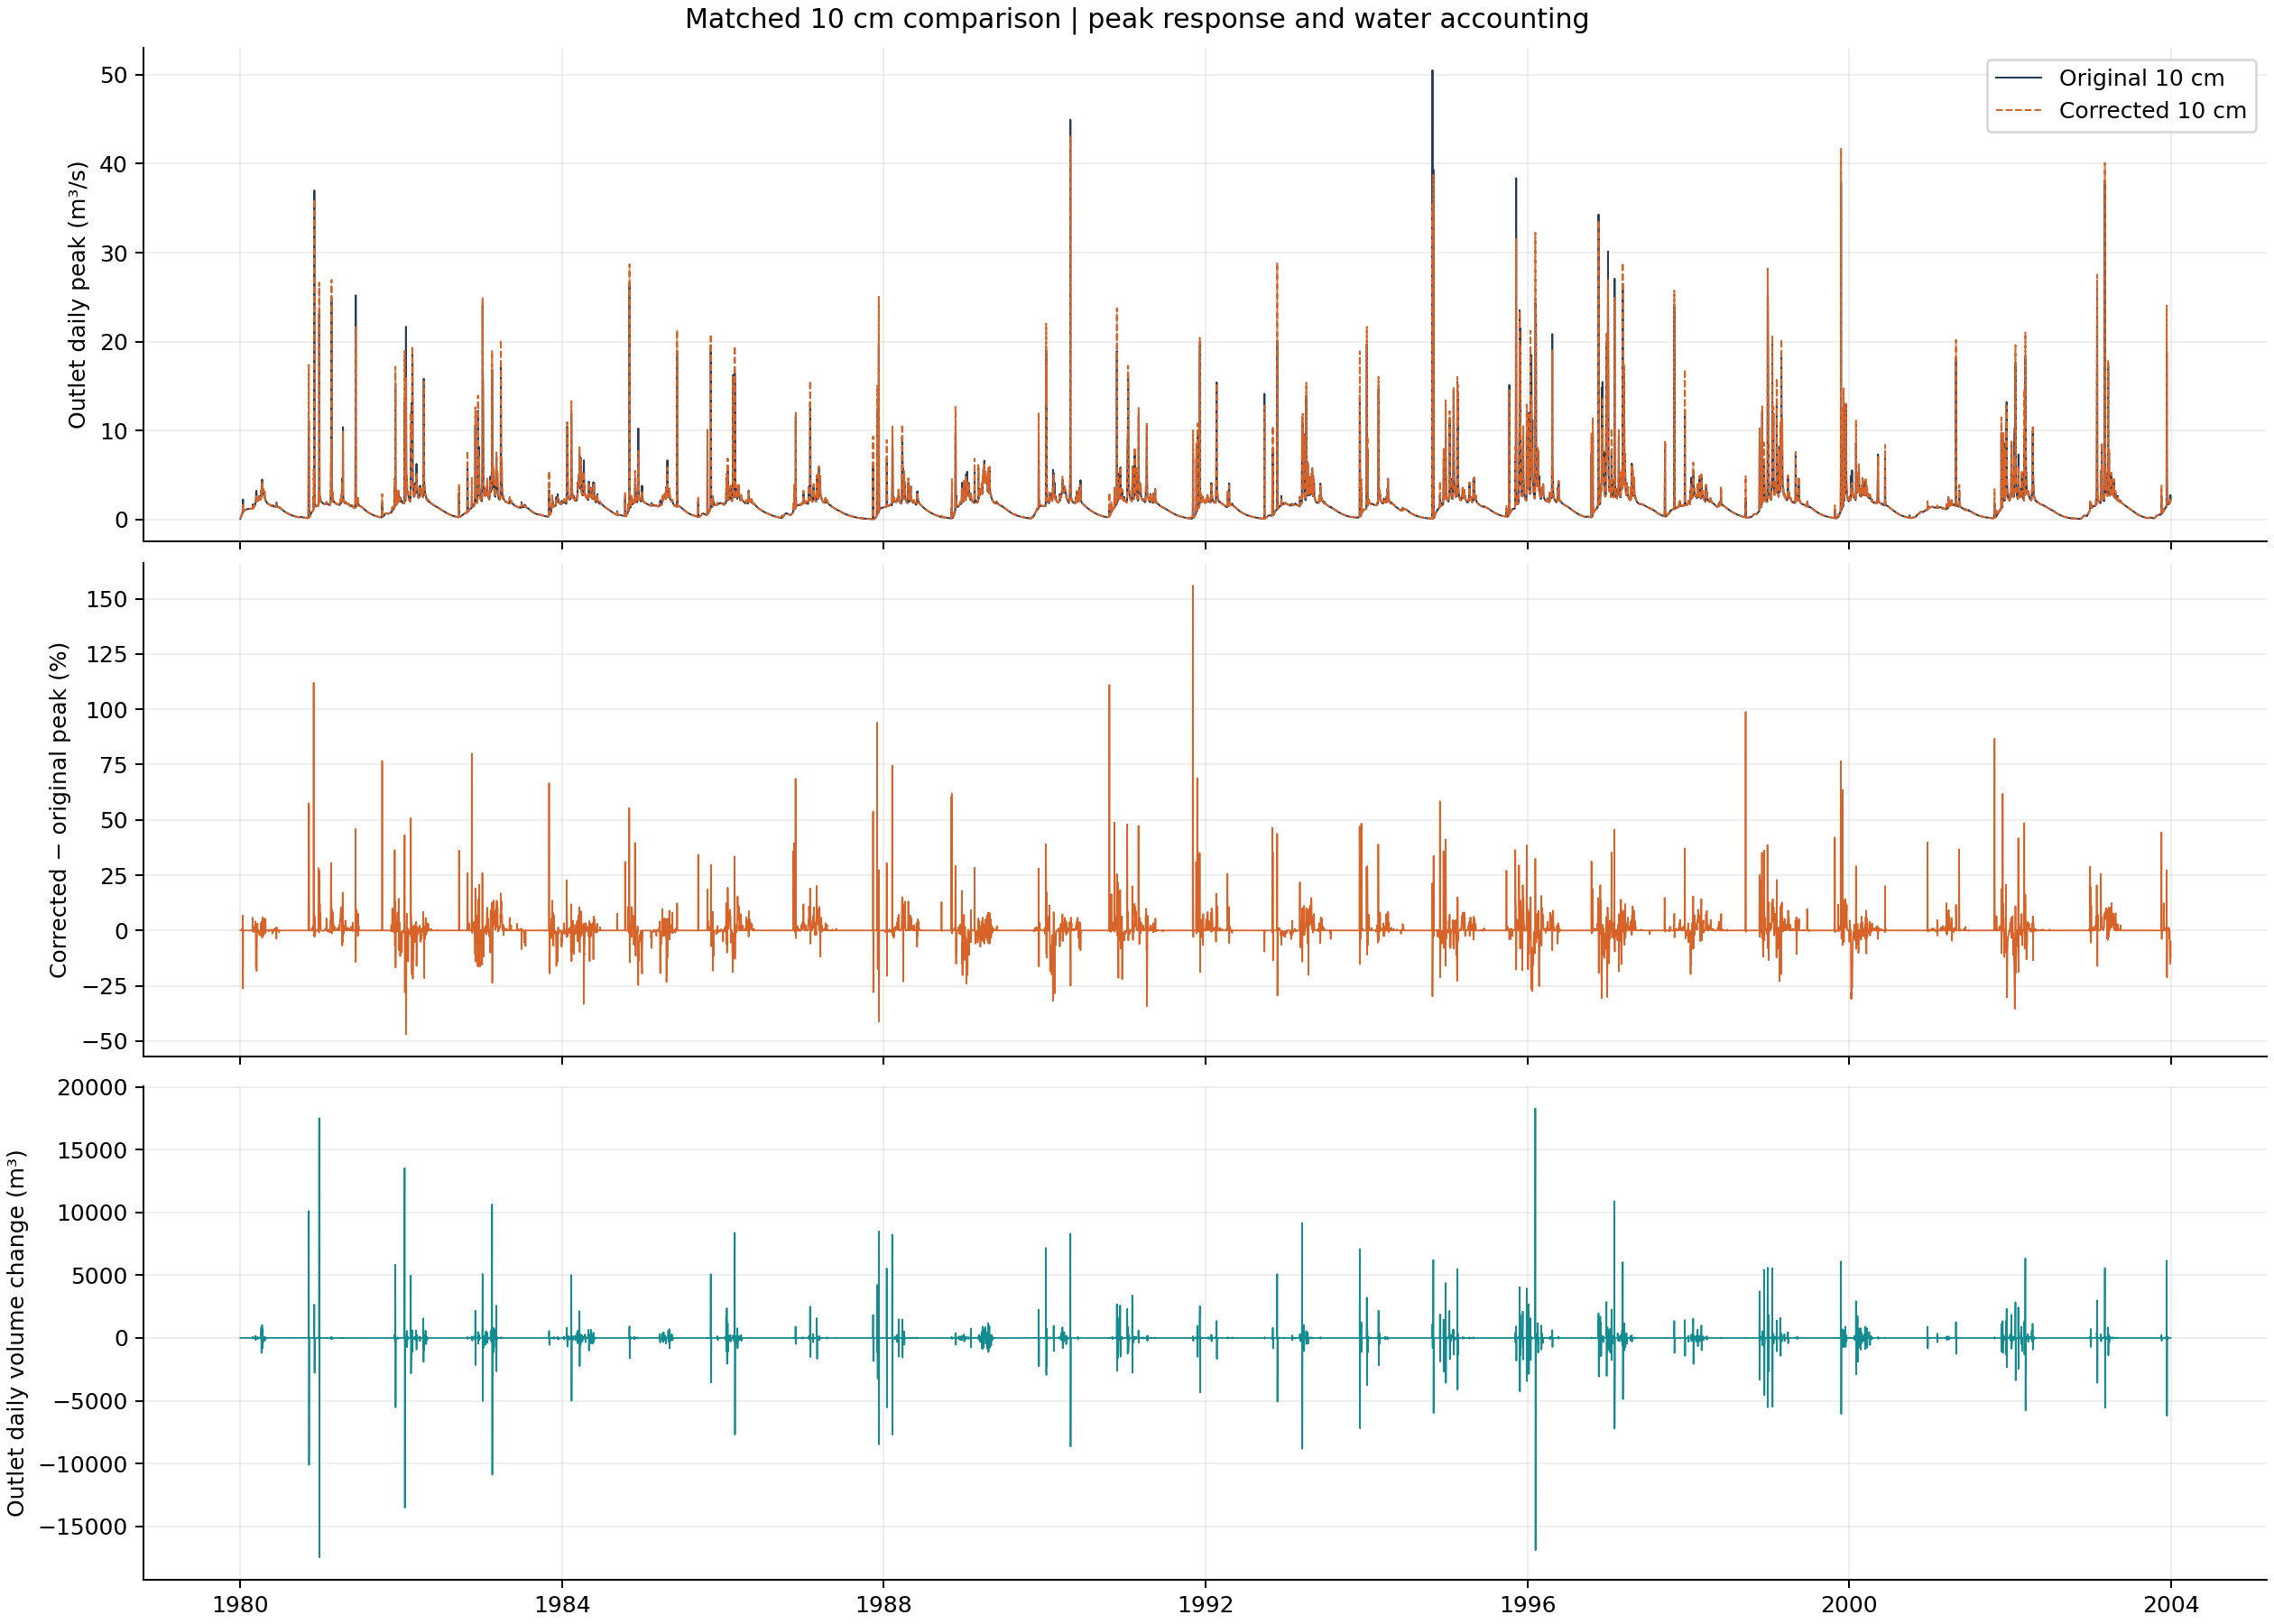
\includegraphics[width=\textwidth,height=.78\textheight,keepaspectratio]{../../work-packages/20261006_warming_rrinit_legacy/artifacts/comparison/figure-2-matched-10cm.png}
\caption{Matched 10 cm original-versus-candidate outlet response. Near-equal
long-term yield does not imply unchanged daily volumes, peak rates or timing.}
\label{fig:matched-builds}
\end{figure}

For smaller outlet events, the three most responsive non-overlapping examples
increase by 111.1\%, 98.9\% and 86.7\%. These use the lower half of original
local peaks (at most 4.087 m$^3$/s), with seven-day separation and
0.1 m$^3$/s prominence, then rank absolute relative build differences.
They are sensitivity examples, not representative or typical-event estimates.
Their narrower, higher curves illustrate why daily yield agreement cannot
validate subdaily routing.

\begin{figure}[p]
\centering
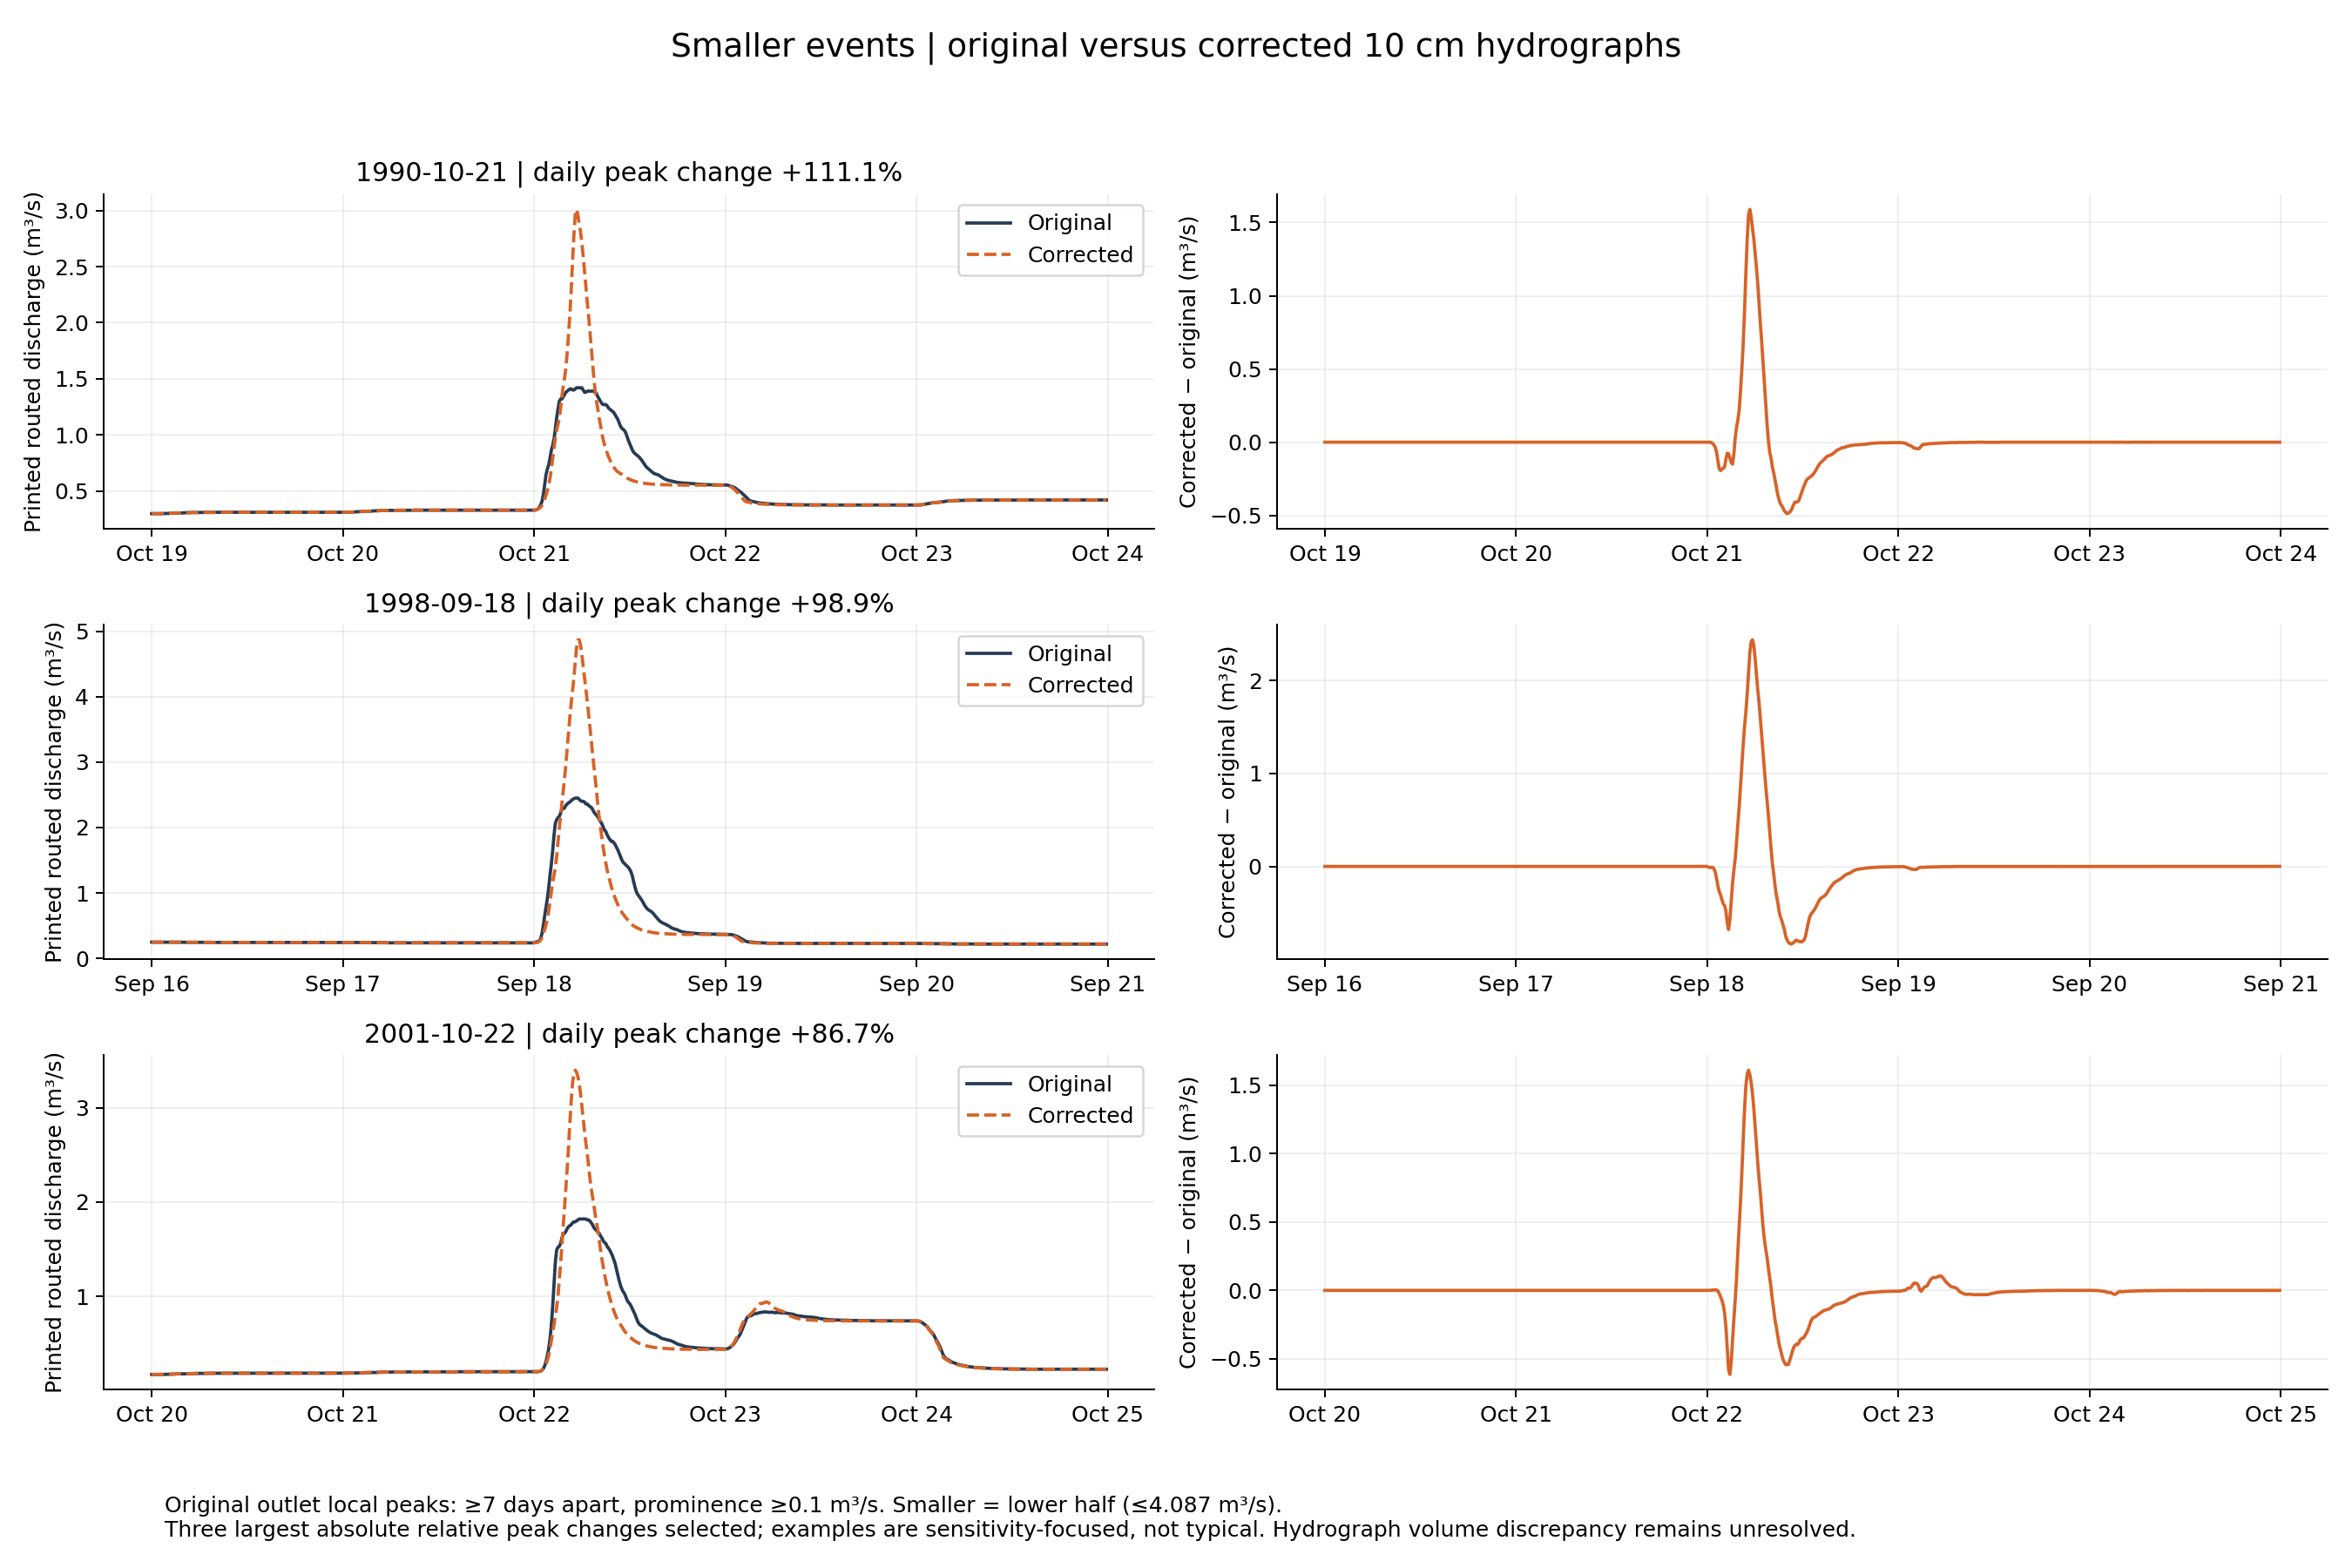
\includegraphics[width=\textwidth,height=.78\textheight,keepaspectratio]{../../work-packages/20261006_warming_rrinit_legacy/artifacts/comparison/figure-4-smaller-events.png}
\caption{Selected smaller-event hydrographs at matched 10 cm inputs. The
candidate can increase peaks. Selection is deliberately sensitivity-focused;
the unresolved hydrograph-volume discrepancy also applies to interpretation.}
\label{fig:small-builds}
\end{figure}
\clearpage

\subsection{Unresolved hydrograph-volume gate}

Agreement between the event report and channel water-balance outflow is exact
at printed precision, but these are ledger measures. In \texttt{WSHCHR},
\texttt{chvol} derives from inflow plus change in storage, separately from the
sampled routed-discharge array \texttt{q1}. Integrating the printed 600-second
hydrograph exposes a distinct inconsistency:

\begin{table}[H]
\centering\small
\caption{Matched 10 cm hydrograph-integral shortfall relative to the
outlet-volume ledger. Printing bounds assume rounding to three significant digits.}
\begin{tabular}{lrrr}
\toprule
Build & Shortfall (million m$^3$) & Fraction of ledger & Rounding bound (million m$^3$) \\
\midrule
Original & 5.889 & 0.4628\% & 2.879 \\
Candidate & 16.810 & 1.3212\% & 2.879 \\
\bottomrule
\end{tabular}
\end{table}

Both shortfalls exceed the conservative cumulative discharge-printing bound.
The candidate increases the discrepancy by about 10.92 million m$^3$.
The five-day October 25--29, 1994 window is more concerning: ledger volumes
are 2,539,873.62 and 2,539,873.33 m$^3$, but the original and candidate curves
integrate to 2,518,796.22 and 2,075,129.58 m$^3$. The deficit increases from
0.83\% to 18.30\%. The lower candidate peak on October 27 therefore cannot
yet be counted as a validated hydrograph improvement. Other selected events
have smaller deficits or a small surplus. Curves have not been normalised
to force closure.

This is an observed routed-output/ledger inconsistency, not proof that the
soil-water balance lost that volume. Its mechanism requires tracing discharge,
inflow, storage and termination bookkeeping. The shared H670 events on
November 20--21, 1985 also retain positive runoff (22.775 and 19.581 m$^3$)
with zero reported peak in both builds; those are pre-existing anomalies,
not newly introduced regressions.

\begin{figure}[p]
\centering
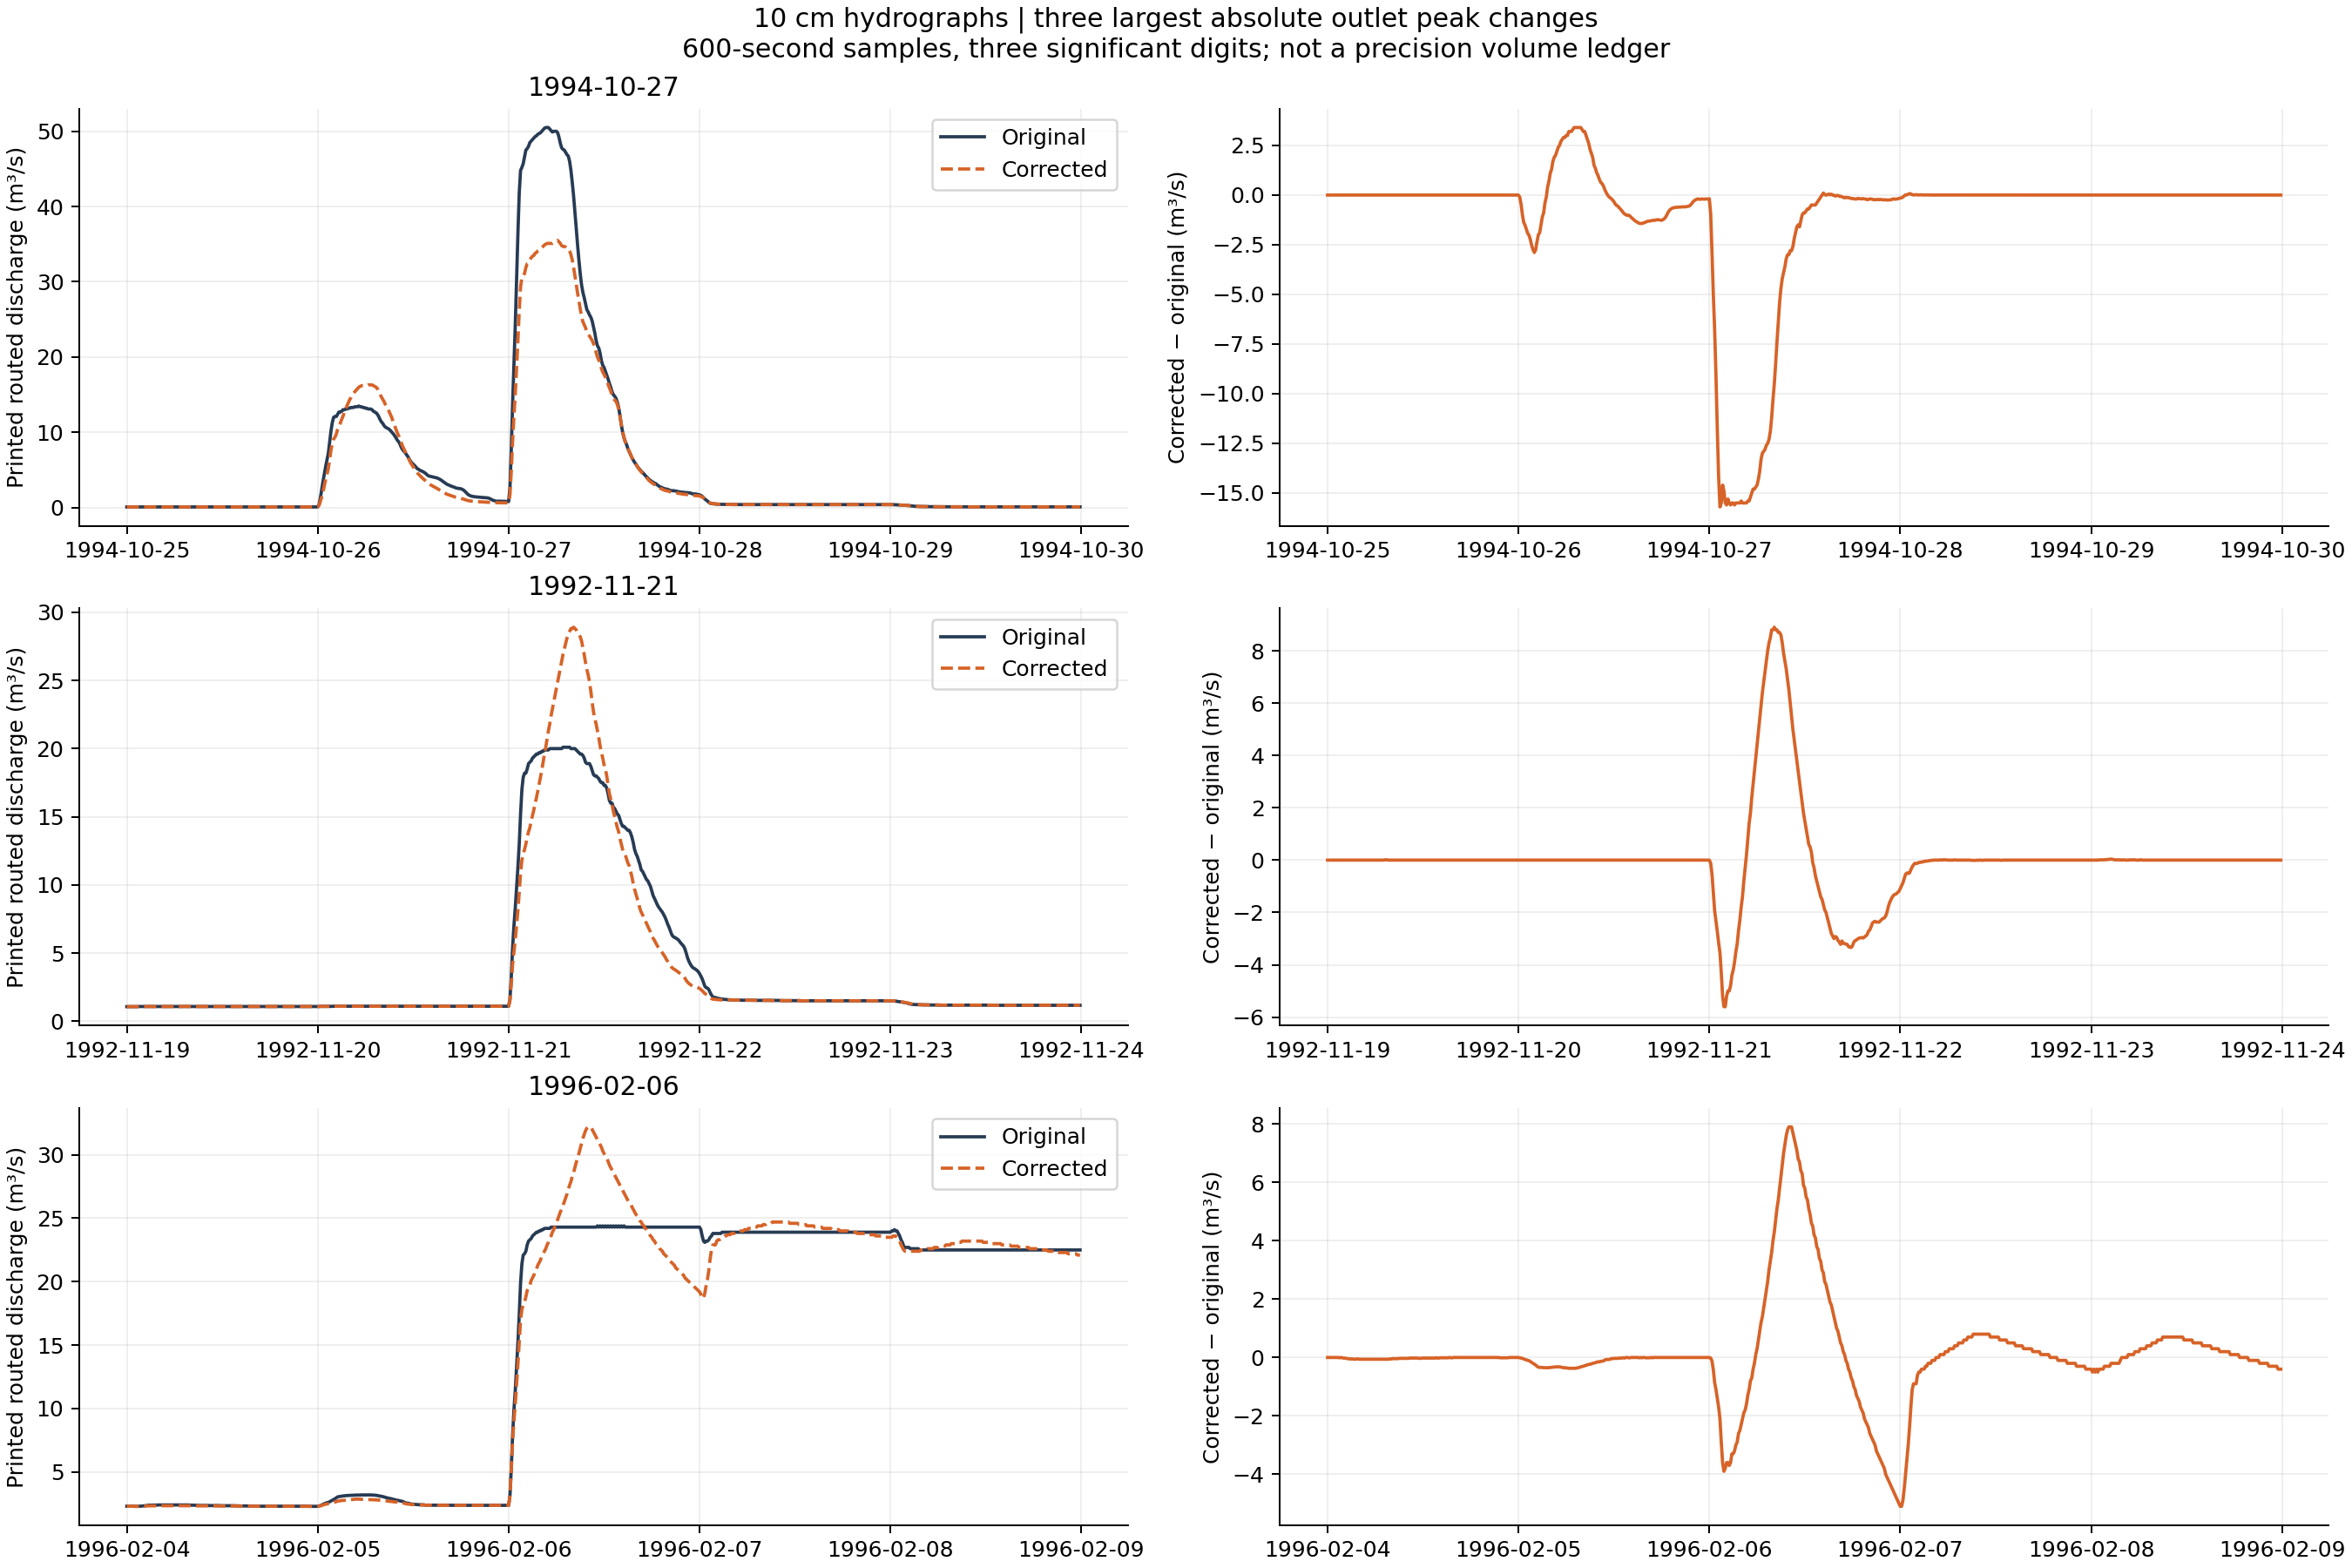
\includegraphics[width=\textwidth,height=.78\textheight,keepaspectratio]{../../work-packages/20261006_warming_rrinit_legacy/artifacts/comparison/figure-3-matched-hydrographs.png}
\caption{Three largest absolute matched outlet-peak changes, separated by
more than seven days. Selection retains both increases and decreases. The
October 1994 window has an 18.30\% candidate hydrograph-volume deficit despite
nearly unchanged ledger volume; lower peaks alone do not validate the repair.}
\label{fig:closure-builds}
\end{figure}
\clearpage

\paragraph{Disposition and stakeholder disclosure.}
Retain physically justified roughness rather than inflate it to suppress a
numerical symptom. The candidate is implemented and has completed these
research comparisons, including input isolation, negative controls and output
readback. It is not a full kinematic-wave repair, does not remove every
mutation sensitivity, and has not passed an unconditional watershed-hydrograph
release gate. Reconcile the sampled-discharge/ledger discrepancy and repeat
the affected acceptance checks before declaring it validated for that use.
Any stakeholder summary should disclose both the mutation improvement and
the adverse closure finding, distinguish daily yield from instantaneous peak,
and state deployment status separately. This report update neither changes
production binaries nor sends an external stakeholder message.
